\chapter{Mathematical Preliminaries}
In this chapter, we build step-by-step preliminaries in mathematical analysis that establish diffusion models. Discrete-time diffusion models are based on Markov chains, which is a stochastic process, and continuous-time are based on stochastic differential equations, both are derived from probability theory. Therefore, we begin by discussing the basics of mathematical analysis needed to develop formal probability theory. From probability theory, we study stochastic processes, stochastic integrals and stochastic differential equations.


\section{Mathematical Spaces}
\subsection{Motivations}

When working with the set of real numbers $\RR$, we are familiar with the absolute value defined $x\in\RR$
\begin{equation}
 \label{equation:number-absolute-value}
 |x| = \begin{cases}
  x, \text{ if } x\ge0 \\
  -x, \text{ if } x < 0.
 \end{cases}
\end{equation}
The distance between two real numbers $x$ and $y$ is $|x-y|$. We also concern about sequences of real numbers with properties such as boundedness and convergence. A sequence $(x_n)_{n\in\NN}\subset\RR$ is bounded if
$$\exists M\in\RR, \forall n\in \NN, |x_n|\le M.$$
The sequence $(x_n)_{n\in\NN}\subset\RR$ converges to a limit $x$ if
$$\forall \epsilon > 0, \exists N\in\NN, \forall n>N, |x_n-x|<\epsilon.$$

These concepts have been generalized to $\RR^d$. For each vector $\xbf=(x_1,\ldots,x_d)\in\RR^d$, the absolute value becomes the norm
\begin{equation}
 \label{equation:vector-norm}
 \|\xbf\| = \sqrt{x_1^2+\ldots+x_2^d}.
\end{equation}
The distance between two vectors $\xbf$ and $y$ is $|\xbf-\ybf|$. The norm is a real number, and it lets us define properties of sequence as in $\RR$. This is actually the evolution of mathematics: mathematicians first work with real-life objects, such as arithmetic numbers or Euclidean geometry shapes, then discover the same pattern with another objects, such as the vectors. Then, they developed an abstract structure covering these objects, ignoring the very details, such as the vector space. The abstraction progress really fulfills the picture of mathematics, and extends mathematics applications. In forthcoming sections, we will see the benefits of following introductory concepts. For example, we can regard a specific class of random variables (see Definition \ref{definition:random-variable}) and stochastic processes (see Definition \ref{definition:stochastic-process}) akin to the real numbers. Such abstractions graciously facilitate to further developments relating to the studied objects.

Motivated enough, we are going to generalize these concepts of norm, distance and convergence in following discussions by three spaces, namely metric space, normed space and Banach space.

\subsection{Metric Space}

\begin{definition}
 Given a set $\Omega$. A function $d:\Omega\times\Omega\to\RR$ is called a \textbf{metric} if it satisfies
 \begin{enumerate}
  \item Non-negativity: $d(x,y)\ge 0,\forall x,y\in\Omega$. The equality holds if and only if $x=y$.
  \item Symmetry: $d(x,y)=d(y,x)$.
  \item Triangle inequality: $d(x,y)+d(y,z)\ge d(x,z)$.
 \end{enumerate}
 The tuple $(\Omega,d)$ is called a \textbf{metric space}\index{metric space}.
\end{definition}

\begin{example}
 \begin{enumerate}
  \item []
  \item Given a set $\Omega$ and a function $d:\Omega\times\Omega\to\RR$ defined by
        $$d(x,y)=\begin{cases}
          1, & \text{ if } x=y     \\
          0, & \text{ if } x\ne y.
         \end{cases}$$
        Then $d$ is a metric
  \item Let $(\Omega, \|\cdot\|)$ be a normed space. Define $$d(x,y) = \|x-y\|, \forall x,y\in\Omega.$$
        Then $d$ is a metric.
 \end{enumerate}
\end{example}

\begin{definition}
 Let $(\Omega, d)$ be a metric space. A subset $A$ of $\Omega$ is said to be \textbf{open}\index{open} if for any $x\in A$, there exists $\epsilon > 0$ such that if a point $y$ having $d(x, y)<\epsilon$, then $y\in A$.
\end{definition}

\begin{definition}
 Let $(\Omega, d)$ be a metric space. A sequence $(x_n)_{n=1}^\infty\subset\Omega$ is said to \textbf{converge}\index{convergence} to $x\in\Omega$ if
 $$\forall \epsilon>0, \exists N>0,\forall n> N, x_n\in B_\epsilon(x).$$
\end{definition}

\begin{definition}
 A metric space $\Omega$ is said to be \textbf{complete} if every convergent sequence in $\Omega$ has the limit in $\Omega$.
\end{definition}

\subsection{Normed Space}

\begin{definition}
 Let $K$ be a filed and $V$ be a vector space over $\mathbb{K}$. A function $\|\cdot\|: V\to \RR$ is called a \textbf{norm}\index{norm} if it satisfies
 \begin{enumerate}
  \item Non-negativity: $\|x\|\ge0,\forall x\in V$. The equality holds if and only if $x=0$.
  \item Absolute homogeneity: $\|\lambda x\| = |k|\cdot\|x\|,\forall x\in V, \lambda\in\mathbb{K}$.
  \item Triangle inequality: $\|x\|+\|y\|\ge \|x+y\|,\forall x,y\in V$.
 \end{enumerate}
 The tuple $(V,\|\cdot\|)$ is called a \textbf{normed space}\index{normed space}.
\end{definition}

\begin{example}
 \begin{enumerate}
  \item []
  \item Regard $\RR^d$ as a real vector space. For each $p\in[1,\infty]$, defined the function $\|\cdot\|_p:\RR^d\to\RR$ for each $\|\xbf\|_p = (x_1,\ldots, x_n)$ by
        \begin{equation}
         \|\xbf\|_p = \begin{cases}
          \left(\sum\limits_{i=1}^d |x_i|^p\right)^{1/p}, & \text{ if } p <\infty \\
          \sup\{x_i, \,\,1\le i \le d\}.,                 & \text{ if } p =\infty
         \end{cases}
        \end{equation}
        Then $\|\cdot\|_p$ is a norm, called the $p$-norm of $\RR^d$.
  \item Regard $\RR^{d\times r}$ as a real vector space. Let function $\|\cdot\|_F: \RR^{d\times r}\to\RR$ be defined for each $\Abf = (a_{ij})\in\RR^{m\times n} $ as
        $$\|A\|_F = \sqrt{\sum\limits_{i=1}^m\sum\limits_{j=1}^na_{ij}^2}.$$
        Then $\|\cdot\|_F$ is a norm, called the Frobenius norm.
 \end{enumerate}
\end{example}

% \begin{theorem}[Cauchy-Schwartz inequality]
%   \label{cauchy-schwartz-inequality}
% \end{theorem}

\subsection{Banach Space}
\begin{definition}
 A \textbf{Banach space}\index{Banach space} is a normed space that is complete with respect to the metric induced by the norm.
\end{definition}

\section{Measure Theory and Integration}
\subsection{Measure Space}
In the normal sense of the word ``measure'', the measure of any interval $I=[a,b]$, in $\RR$ coincides with the length $\ell(I)=|b-a|$. Similarly, the area of a square $S = [a_1,b_1]\times [a_2,b_2] = I_1\times I_2$ in $\RR^2$ is $\ell(I_1)\cdot\ell(I_2)$. More generally, given intervals $I_k = [a_k,b_k], k = 1,\ldots, n$, the volume of the box $B= I_1\times \ldots \times I_n$ in  $\RR^n$ is $\prod\limits_{k=1}^n \ell(I_k)$. Measure theory generalizes the length, area and volume to other measures on other abstract sets $\Omega$ rather than $\RR^n$. Moreover, this branch of real analysis establishes the class of measurable subsets of $\Omega$. To see the reason for this diligent work of mathematicians on measure theory, let us take an example on the measure of length. As in ordinary contexts, the length $\ell(E)$ of any subset $E$ of $\RR$, if exists, is required to satisfy

\begin{enumerate}
 \item Non-negativity: $\ell(E) \ge 0$.
 \item If $E\subset F\subset \RR$, then $\ell(E)\le \ell(F)$.
 \item If $E=[a,b]$, then $\ell(E) = |b-a|$.
 \item Translation invariance: for any $x\in\RR$, $\ell(E+x) = \ell(E)$.
 \item If $E$ can be divided to a collection of disjoint intervals $\{I_k\}_{k\in N}$, assuming that $\ell(\varnothing) = 0$, then $\ell(E) = \sum\limits_{k=1}^\infty \ell(I_k).$
\end{enumerate}

We will prove that our intuitive length measure cannot be applied for all subsets of $\RR$ \cite{vitali1905sul}.

\begin{proposition}
 If there exists $\ell : 2^\RR \to [0,\infty]$ satisfying
 \begin{enumerate}[label=(\arabic*)]
  \item If $E=[a,b]$, then $\ell(E) = |b-a|$. Also assume that $\ell(\varnothing) = 0$.
  \item If $E\subset F\subset \RR$, then $\ell(E)\le \ell(F)$.
  \item Translation invariance: for any $x\in\RR$, $\ell(E+x) = \ell(E)$.
  \item If $E$ can be divided to a collection of disjoint intervals $\{I_k\}_{k\in N}$, then $\ell(E) = \sum\limits_{k=1}^\infty \ell(I_k).$
        % \item (Derived from (2) and (4)) for any collection  measurable sets $\{A_k\}_{k=1}^{\infty}$,
        %       $$\ell\left(\bigcup\limits_{k=1}^{\infty} A_k\right) \le \sum_{k=1}^{\infty} A_k.$$
 \end{enumerate}
 Then $\ell(E) = 0, \forall E\in 2^\RR$.
\end{proposition}

\begin{proof}
 By (2), we have $\ell((0,1])\le \ell([0,1]) = 1$. Let us define an equivalence relation \index{equivalence relation} on $(0,1]$ as
 $$x\sim y \Leftrightarrow x-y\in\QQ.$$
 Clearly, for any $x\in (0,1]$, we have the equivalence class
 $$[x] = \{y\in(0,1] : x-y\in \QQ\} = \{x+q: q\in \QQ, x+q\in (0,1]\}.$$
 Denote by $N\in\NN\cup\{\infty\}$ the number of equivalence classes. Choose an element $x_n$ from the $n$-th equivalence class, where $1\le n\le N$\footnote{We have made use of the Axiom of Choice}. Clearly all the $x_n, n\in1,\ldots, N$ are distinct.

 Let $A=\{x_k\}_{k=1}^N\subset(0,1]$ and $(q_n)_{n=1}^\infty$ be a numeration of $\QQ\cap(-1,1]$\footnote{The set of rational number $\QQ$ is countable}. Also, let $A_n = A + q_n$ for any $n\in\NN$. We claim that if $n\neq m$, then $A_n\cap A_m = \varnothing$. We will prove the contrapositive statement. Suppose that there exists $x\in A_n\cap A_m$, then $x=a_n + q_n = a_m + q_m$, where $a_n\in A_n$ and $a_m\in A_m$. Therefore,
 $$a_n-a_m = q_m-q_n\in \QQ,$$
 which implies that $a_n\sim a_m$. Hence, $a_n$ and $a_m$ are presentations of a single equivalent class, or $n=m$.

 On the other hand, $(0,1] \subset \bigcup\limits_{n=1}^\infty A_n \subset (-1,2]$.

 By (3) and (4),
 $$\ell((-1,2]) = \ell((-1,0]) + \ell((0,1]), \ell((1,2]) = 3\ell((0,1]).$$

 By (3), we have

 $$\ell(A_n) = \ell (A), \forall n\in\NN.$$

 By (4) and the previous implications,
 $$\ell((0,1]) \le \ell\left(\bigcup\limits_{n=1}^\infty A_n\right) = \sum\limits_{k=1}^{\infty} \ell(A_k) = \sum_{k=1}^{\infty} \ell(A) \le 3\ell((0,1]).$$

 This implies $\ell(A)=0$, and also $\ell((0,1])=0$. Therefore,

 $$\ell(\RR) = \ell\left(\bigcup\limits_{m\in\ZZ}(m,m+1] \right) = \sum\limits_{m\in\ZZ} \ell((m,m+1])= \sum\limits_{m\in\ZZ} \ell((0,1]) = 0.$$

 Thus, $\ell$ coincides with the zero function. However, this measure of length is unavailing.
\end{proof}


A measure space is the initial model to measure theory. Consider the following real-life example.

\begin{example}
 A farmer has a rectangular land whose width and length are both $100\,m$. The coordinated representation of the land is $\Omega=[0,100]\times[0,100]$. The farmer allocates a region to build a warehouse, whose shape is not restricted to be a rectangle. To approximate the area of this region, the farmer divides it into disjoint rectangular subregions and sums of the areas.
\end{example}

A region is a set of $\Omega$. We know that maybe some subsets of $\Omega$ cannot be measured. Let $\F\subset2^\Omega$ be the family of all measurable subsets of $\Omega$. The area of whole land is known by the farmer i.e. $\Omega\in\F$. On the other hand, if we can measure the area of the warehouse, the rest region's area can also be measured. Motivated by the context, the set of measurable regions as above is defined formally as a $\sigma$-algebra, as below.

\begin{definition}
 \label{definition:sigma-algebra}
 Given a set $\Omega$. A collection of subsets $\F$ of $\Omega$ is called a \textbf{$\sigma$-algebra}\index{$\sigma$-algebra} if
 \begin{enumerate}
  \item $\varnothing, \Omega\in\F$;
  \item If $A\in\F$, then $A^c\in\F$;
  \item If $A_1,A_2,\ldots\in\F$, then $A_1\cup A_2\cup\ldots\in\F$.
 \end{enumerate}
 The pair $(\Omega, \F)$ is called a \textbf{measurable space}\index{measurable space}.
\end{definition}

Definition \ref{definition:sigma-algebra} models measurable objects to be a collection $\F$ of subsets of a given set $\Omega$. Before the definition of a measure, we consider some examples and analytically derived theorems.

\begin{example}
 \label{example:1}
 Given a set $\Omega$, then $\{\varnothing, \Omega\}$ and the power set $2^\Omega$ are two trivial $\sigma$-algebras. Let $\Omega=\{1,2,3\}$, the collection $\F=\{\varnothing,\Omega, \{1\}, \{2,3\}\}$ is a $\sigma$-algebra on $\Omega$.
\end{example}

\begin{proposition}
 Let $\{\F_\alpha\}_{\alpha\in I}$ be an arbitrary family of $\sigma$-algebras on $\Omega$. Then the intersection $\F=\bigcap\limits_{\alpha\in I}\F_\alpha$ is a $\sigma$-algebra.
\end{proposition}

\begin{proof}
 We will check that $\F$ three conditions for a $\sigma$-algebra.

 Since $\varnothing,\Omega\in\F_\alpha,\forall\alpha\in I$, we have $\varnothing,\Omega\in\bigcap\limits_{\alpha\in I}\F_\alpha$.

 If $A\in\bigcap\limits_{\alpha\in I}\F_\alpha$, then $A\in \F_\alpha,\forall\alpha\in I$, leading to $A^c\in \F_\alpha,\forall\alpha\in I$. Hence, $A^c\in\bigcap\limits_{\alpha\in I}\F_\alpha.$

 Finally, if $A_i\in\F_\alpha,\forall i\in\ZZ^+,\forall \alpha\in I$, then $\bigcup\limits_{i\in\ZZ^+}A_i\in\F_\alpha,\forall\alpha\in I$. Therefore,
 $\bigcup\limits_{i\in\ZZ^+}A_i\in\bigcap\limits_{\alpha\in I}\F_\alpha.$
\end{proof}

\begin{remark}
 The union of $\sigma$-algebras on $\Omega$ is not necessarily a $\sigma$-algebra. For example,
 $$\F_1=\{\varnothing,\Omega, \{1\}, \{2,3\}\} \text{ and } \F_2=\{\varnothing,\Omega, \{2\}, \{1,3\}\}$$
 are two $\sigma$-algebras on $\Omega=\{1,2,3\}$, but
 $$\F=\F_1\cup\F_2=\{\varnothing,\Omega,\{1\},\{2\},\{2,3\},\{1,3\}\}$$ is not, since $\{3\}=\{2,3\}\cap\{1,3\}\notin \F$.
\end{remark}

Having mentioned in Example \ref{example:1}, any collection $\C$ of subsets of $\Omega$, has a trivial $\sigma$-algebra $2^\Omega$ that contains $\C$ i.e. $\C\subset2^\Omega$. Therefore, there exists the smallest $\sigma$-algebra containing $\C$.

\begin{theorem}
 \label{theorem:generated-sigma-algebra}
 Given a set $\Omega$ and a collection of its subsets $\C$, there exists the smallest $\sigma$-algebra containing $\C$, denoted by $\sigma(\C)$, given by
 $$\sigma(\C)=\bigcap\limits_{\alpha\in I}\F_\alpha,$$
 where $\{\F_\alpha\}_{\alpha\in I}$ is the set of $\sigma$-algebras containing $\C$. We also called $\sigma(\C)$ to be the $\sigma$-algebra generated by $\C$.
\end{theorem}

\begin{proof}
 Since $\sigma(\C)$ itself is a $\sigma$-algebra containing $\C$ so $\sigma(\C)\in\{\F_\alpha\}$, leading to

 $$\bigcap\limits_{\alpha\in I}\F_\alpha\subset \sigma(\C).$$

 Moreover, $\bigcap\F_i$ is also a $\sigma$-algebra containing $\C$ and $\sigma(\C)$ is the smallest one, hence

 $$\sigma(\C)\subset\bigcap\limits_{\alpha\in I}\F_i.$$

 Thus, $\sigma(\C)=\bigcap\limits_{\alpha\in I}\F_i$.
\end{proof}

\begin{remark}
 Theorem \ref{theorem:generated-sigma-algebra} tells us that a collection of measurable subsets can be extended to a $\sigma$-algebra. For example, a collection $\C=\{\{1\}\}$ of subsets of $\Omega=\{1,2,3\}$ generates the $\sigma$-algebra
 $$\F=\{\varnothing,\Omega,\{1\},\{2,3\}\}.$$
\end{remark}

\begin{figure}[ht]
 \centering
 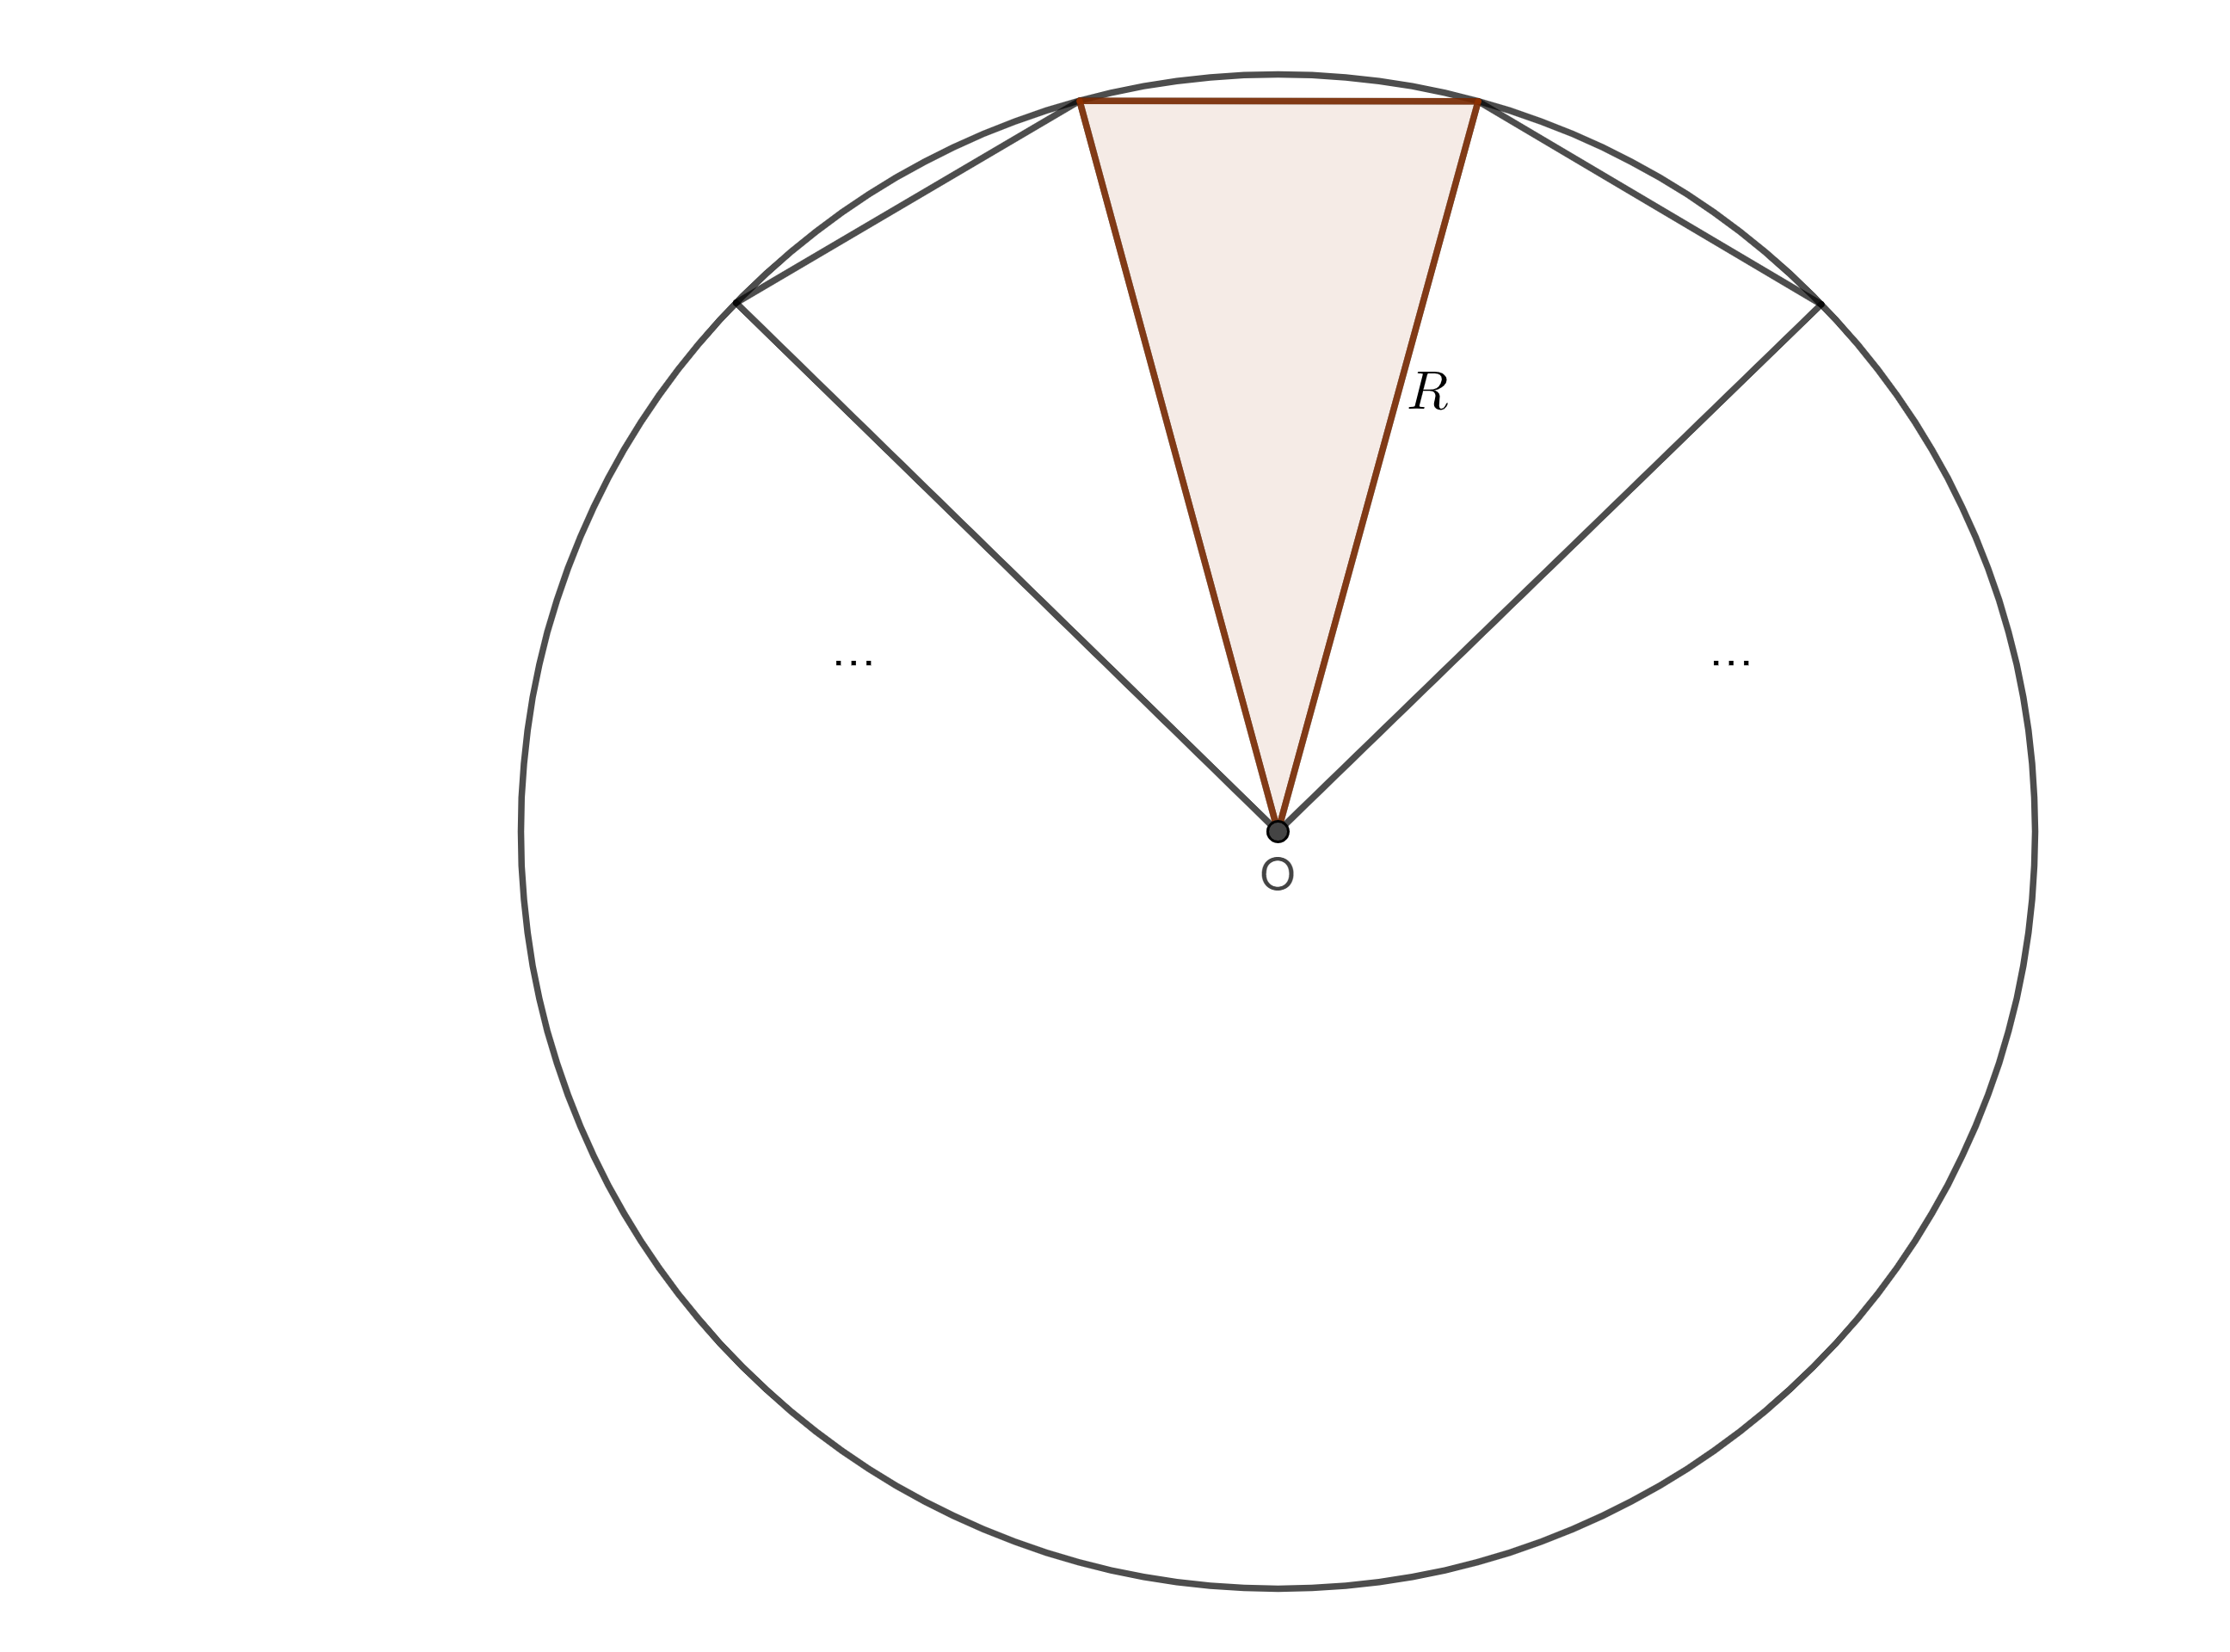
\includegraphics[width=0.4\linewidth]{img/circle.png}
 \vspace{0.5cm}
 \caption[Circle area approximation]{The area of a circle can be calculated by dividing it into equal isosceles triangles. As the number of triangles tends to infinity, the sum of bottom sides tends to the perimeter $2\pi R$ of the circle and the attitude of a triangle tends to $R$. Hence, the area is $A=\dfrac{1}{2}(2\pi R)R=\pi R^2$.}
 \label{figure:circle}
\end{figure}

\begin{definition}
 Given a measurable space $(\Omega,\F)$, a function $\mu:\F\to\RR$ is called a \textbf{measure}\index{measure} if it satisfies
 \begin{enumerate}
  \item Non-negativity: $\mu(A)\ge0,\forall A\in\F.$
  \item $\mu(\varnothing)=0$.
  \item Countable additivity: if $\{A_i\}_{i=1}^\infty\subset\F$ contains pairwise disjoint elements, then
        $$\mu\left(\bigcup\limits_{i=1}^\infty A_i\right)=\sum\limits_{i=1}^\infty \mu(A_i).$$
        The triplet $(\Omega,\F,\mu)$ is called a measure space.
 \end{enumerate}
\end{definition}

% \begin{theorem}[Properties of a measure]
%   \begin{enumerate}
%     \item[]
%     \item Monotonicity\index{monotonicity}: if $A\subset B$, then $\mu(A)\le\mu(B)$.
%   \end{enumerate}
% \end{theorem}

\begin{example}
 \begin{enumerate}
  \item []
  \item Consider the measurable space $(\RR, \B(\RR))  $. The function of taking the length of open intervals on the real line
        $$\mu((x,y))=|y-x|,\forall x,y\in\RR,$$
        which an assumption that $\mu(\varnothing)=0$, is a measure. Three properties of a measure are satisfied trivially.
  \item Consider the measurable space $(\RR, \F)$, where $\F$ is any $\sigma$-algebra on $\RR$. Given $a\in\RR$. The indicator function $\mathbf{1}_a: \F\to\{0,1\}$ given by
        $$\begin{cases}
          \mathbf{1}_a(X)=1, & \text{ if } a\in X \\
          \mathbf{1}_a(X)=0, & \text{ otherwise }
         \end{cases}$$
        is a measure. We already have $\mathbf{1}_a(X)\ge0, \forall a\in X$. Let us check the other two properties of a measure for this function.
        \begin{itemize}
         \item Since $a\notin\varnothing$, we have $\mathbf{1}_a(\varnothing)=0$.
         \item For disjoints $X_1,X_2,\ldots$ it cannot be the case that there are two of them contain $a$. If $a\notin X_k,\forall k\in\ZZ^+$, then countable additivity holds since both sides are zero. Otherwise, if there exists $k\in \ZZ^+$ such that $a\in X_k$, then it follows that $$a\notin X_\ell, \forall \ell\ne k,$$ implying both sides are one.
        \end{itemize}
 \end{enumerate}
\end{example}

Given measure spaces $(\Omega,\F,\mu)$ and $(\Gamma,\G,\nu)$, we also concern about which pair $(x,\gamma)\in\Omega\times\Gamma$ that can be measured and how to measure them.

\begin{definition}
 Let $(\Omega,\F,\mu)$ and $(\Gamma,\G,\nu)$ be measure spaces. The \textbf{product $\sigma$-algebra}\index{product $\sigma$-algebra} $\F\otimes\G$ on $\Omega\times\Gamma$ is given by
 $$\F\otimes\G=\sigma(\{A\times B : A\in\F,B\in\G\}).$$
\end{definition}

\begin{definition}
 Let $(\Omega,\F,\mu)$ and $(\Gamma,\G,\nu)$ be measure spaces. The \textbf{product measure}\index{product measure} $\lambda(A\times B)$ on $\F\otimes\G$, where $A\in\F,B\in\G$ is given by
 $$\lambda(A\times B)=\mu(A)\nu(B)$$
\end{definition}

\begin{example}
 The measure of area $\mu$ in a two-dimensional space can be thought of as the product of two identical measures of length $\lambda$ in a one-dimensional space. Given two intervals $[a,b]$ and $[c,d]$, the equality
 $$\mu([a,b]\times [c,d])=\lambda([a,b])\cdot\lambda([c,d]),$$
 meets our intuition about the area of a rectangle. Here it also suggests that a rectangle with one size to be zero has area measure zero.
\end{example}

\begin{definition}
 \label{definition:property-almost-everywhere}
 Let $(\Omega, \F, \mu)$ be a measure space. A property $\P:\Omega\to\{\texttt{true},\texttt{false}\}$ is said to hold \textbf{almost everywhere}\index{almost everywhere} with respect to $\mu$, abbreviated by $\mu$-a.e. if
 $$\mu\left(\left\{x\in\Omega : \neg \P(x)\right\}\right) = 0.$$
\end{definition}

\subsection{Borel \texorpdfstring{$\sigma$}{σ}-algebra}

\begin{definition}
 Let $\mathcal{X}$ be a metric space. The $\sigma$-algebra $\B(\mathcal{X})$ \textbf{generated}\index{generated $\sigma$-algebra} by open subsets of $\mathcal{X}$ is called the Borel $\sigma$-algebra on $\mathcal{X}$. Each element in $\B(\mathcal{X})$ is called a Borel subset of $\mathcal{X}$.
\end{definition}

Borel $\sigma$-algebra is an essential class of $\sigma$-algebra. Borel $\sigma$-algebras on real vector spaces $\RR^d$ is later used to define random variables. These associated Borel $\sigma$-algebras can be thought of as containing all Lebesgue measurable and well-behave subsets of $\RR^d$.

\begin{proposition}
 \label{proposition:equivalent-borel-core}
 The Borel $\sigma$-algebra $\B(\RR)$ is generated by one of the following collections
 \begin{enumerate}[label=(\alph*)]
  \item the collection of all closed subsets of $\RR$;
  \item the collection of all intervals of the form $(-\infty,b]$;
  \item the collection of all intervals of R of the form $(a,b]$.
 \end{enumerate}
\end{proposition}

\begin{proof}
 Let $\B_1$, $\B_2$, and $\B_3$ be the $\sigma$-algebra generated by the collections of sets in parts (a), (b), and (c) of the proposition. We will show that
 $$\B(\RR)\supset \B_1 \supset \B_2 \supset \B_3 \supset \B(\RR).$$

 Since $\B(\RR)$ includes the family of open subsets of $\RR$ and is closed under complementation, it includes the family of closed subsets of $\RR$; thus it includes $\B_1$.

 The sets of the form $(-\infty,b]$ are closed and so belong to $\B_1$; consequently $\B_1 \supset \B_2$.

 Since $(a,b]=(-\infty,b]\cap(-\infty,a]^c$, each set of the form
 $(a,b]$ belongs to $\B_2$; thus $\B_2 \supset \B_3$.

 Finally, note that each open intervals of $\RR$ is the union of a sequence of sets of the form $(a,b]$ and that each open subset of $\RR$ is the union of a sequence of open intervals. Thus, each open subset of $\RR$ belongs to $\B_3$, and so $\B_3 \supset \B(\RR)$.
\end{proof}

\begin{proposition}
 The Borel $\sigma$-algebra $\B(\RR^d)$ is generated by one of the following collections
 \begin{enumerate}[label=(\alph*)]
  \item the collection of all closed subsets of $\RR^d$;
  \item the collection of all closed half-space of the form $\{(x_1,\ldots,x_d): x_1\le b_1,\ldots, x_d\le b_d\}$;
  \item the collection of all boxes of the form $\{(x_1,\ldots,x_d): a_1\le x_1\le b_1,\ldots,a_d\le x_d\le b_d\}$.
 \end{enumerate}
\end{proposition}

% \subsection{Lebesgue Measure}

% Lebesgue measure is the generalization of the length of subsets of $\RR$, and also the area and the volume for higher dimensional spaces. Let us denote Lebesgue measure on $\RR^n$ by $\lambda$, which we will construct later. Developed from the ordinary context of the length, area and volume, Lebesgue measure is required to satisfy translation invariance, i.e. for any $\lambda$-measurable set $A$ and $x\in\RR^n$, we have

% \begin{equation}
%   \label{equation:definition:translation-invariance}
%   \mu(A+x) = \mu(A).
% \end{equation}

% For any interval $I=(a,b)$ or $I=[a,b]$, define $\ell(I) = |b-a|$. For any subset $E\subset\RR$, the Lebesgue outer measure is defined as

% \begin{equation}
%   \label{equation:definition:lebesgue-outer-measure}
%   \lambda^*(E) = \inf\left\{\sum\limits_{k=1}^\infty\ell(I_k) : (I_k)_{k\in\NN} \text{ is a sequence of interval such that } E\subset\bigcup \sum\limits_{k=1}^\infty I_k\right\}.
% \end{equation}

\subsection{Measurable Map}

A measurable function is a function between the underlying sets of two measurable spaces that preserves the structure of the spaces: the preimage of any measurable set is measurable. This is in direct analogy to the definition that a continuous function between topological spaces preserves the topological structure: the preimage of any open set is open. Measurable functions are later used in the definition of the Lebesgue integral. In probability theory, a measurable function on a probability space is known as a random variable.

\begin{definition}
 Given two measurable spaces $(\Omega, \F)$ and $(\Gamma,\G)$. A map $f:\Omega\to\Gamma$ is said to be $(\F,\G)$-\textbf{measurable}\index{measurable map}  if
 $$f^{-1}(G)\in\F,\forall G\in \G.$$
\end{definition}

\begin{proposition}
 \label{preposition:preimage-of-a-measurable-map-over-the imaged-sigma-algebra-is-a-sigma-algebra}
 Given two measurable spaces $(\Omega, \F)$ and $(\Gamma,\G)$. If a map $f:\Omega\to\Gamma$ is $(\F\to\G)$-measurable, then the collection $\{f^{-1}(G) : G\in\G\}$ is a sub-$\sigma$-algebra of $\F$. Moreover, it is the smallest $\sigma$-algebra with respect to which $f$ is measurable.
\end{proposition}

\subsection{Lebesgue Integral}

Those familiar with calculus are acquainted with the Riemann integral, which deals with integrating functions defined on real numbers using a partition-based approach.

\begin{definition}
 \begin{enumerate}
  \item []
  \item Given an interval $[a,b]$, a \textbf{partition} $P$ of $[a,b]$ is a finite collection of distinct points in $[a, b]$, including the endpoints
        $$P[a,b]:=\{a=t_0<t_1<\ldots<t_{m}=b\}.$$
        If the interval $[a,b]$ is predefined, we can denote the partition by $P$.
  \item The mesh size of $P$ is
        $$|P|:=\max\limits_{0\le k\le m-1}|t_{k+1}-t_k|.$$
  \item For fixed $0\le\lambda\le 1$ and a partition $P$ of $[0,T]$, set
        $$\tau_k = (1-\lambda) t_k + \lambda t_{k+1},\,\, k=0,\ldots,m-1.$$
        This point lies in the interval $[t_k,t_{k+1}]$.
 \end{enumerate}
\end{definition}

Let $f: [a,b]\to\RR$ be a bounded, continuous function. Geometrically, the Riemann integral of $f$ is equals to the area of the region bounded by the horizontal axis and $f$, and the lines $x=a$ and $x=b$. Let
$$P^n=\{a=t^n_0<t^n_1<\ldots<t^n_{m_n}=b\}, n\in\NN$$ be partitions on $[a,b]$ such that $|P^n|\to 0$ as $n\to\infty$. Using the Fundamental Theorem of Calculus, the Riemann integral of $f$ is

\begin{equation}
 \label{equation:definition:riemann-integral}
 \int\limits_a^b f(x)\d  x = \lim\limits_{n\to\infty}\sum\limits_{k=0}^{m_n-1}f(\tau_k^n)(t_{k+1}^n-t_k^n) = F(b)-F(a),
\end{equation}

where $F$ is an antiderivative of $f$. In the above definition, we use the limits when the mesh size of the partitions $\{P^n\}_{n\in\NN}$ tends to infinity to approximate the area. However, a challenge for Riemann integral raises in higher-dimensional case. For example, consider another function $g: D\to\RR$, where $D$ is a domain in $\RR^2$. To approximate the volume bounded by $g(D)$ and the plane $\RR^2$, we have to define explicitly partitions $\{P^n\}_{n\in\NN}$ on $D$ such that the area of each subdomain of a partition tends to $0$ as $n$ tends to infinity. When $D\in\RR^3$, redefinition is required, and so on.

The mathematician Henri Lebesgue came up with a novel approach for general dimensional cases. A comparison with Riemann integral in the real-input case is illustrated in Figure \ref{figure:schilling}. His idea is to partition the range $f(D)\subset\RR$ instead of the domain $D$. Suppose that $f:D\to\RR$ is bounded on $D$. Consider partitions $$P^n=\left\{\inf\limits_{x\in D} f=t^n_0<t^n_1<\ldots<t^n_{m_n}=\sup\limits_{x\in D} f\right\}, n\in\NN$$ such that $|P^n|\to 0$ as $n\to\infty$. For each $k\in\{0,\ldots,m_n-1\}$ define

\begin{figure}
 \centering
 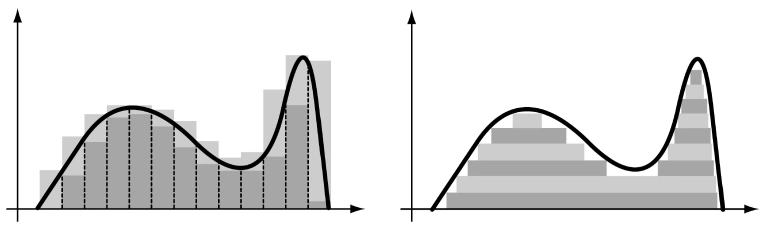
\includegraphics[width=0.75\linewidth]{img/riemann-vs-lebesgue.png}
 \vspace{0.5cm}
 \caption[Riemann and Lebesgue approximations]{Riemann and Lebesgue approximations \cite{schilling2017measures}}
 \label{figure:schilling}
\end{figure}

$$L_k^n=\{x\in\KK \,|\, t_k^n\le f(x)\le t_{k+1}^n\}.$$

Then the following approximation is usable for the area bounded by $f(D), y=0, x=a$ and $x=b$ for $D=[a,b]$, which coincides with Riemann integral.

\begin{equation}
 \label{example:lebesgue-partition}
 I_n=\sum\limits_{k=0}^{m_n-1}(t_{k+1}-t_k)\lambda(L_k^n).
\end{equation}

The additional requirement is that each $L^n_k$ is Lebesgue measurable. In Riemann integral, the function $f$ is required to be discontinuous at finite number of points, which is less general than Lebesgue measurability. Furthermore, Equation \ref{example:lebesgue-partition} can be generalized for abstract set $\Omega$ rather than $\RR^d$, its $\sigma$-algebra $\F$ and a measure $\mu$. In such measure space $(\Omega, \F, \mu)$, we will formally construct the Lebesgue integral for each measurable function $f:\Omega\to\RR$. The idea is to approximate $f$ by the limit of a sequence of steps function $(f_n)_{n\in\NN}$.

\begin{definition}[Step function]
 Let $(\Omega, \F, \mu)$ be a measure space. A function $f:\Omega\to\RR$ is a \textbf{step function}\index{step function} if there exists $\{A_n\}_{n=1}^N\subset\Omega$ and $\{c_n\}_{n=1}^N\subset\RR$ such that
 \begin{equation}
  f(x)=\sum\limits_{i=1}^nc_i\mathbf{1}_{A_i}(x).
 \end{equation}
\end{definition}

\begin{proposition}
 \label{proposition:standard-representation-of-a-step-function}
 Let $(\Omega, \F, \mu)$ be a measure space. Let $f:\Omega\to(0,\infty)$ be a positive step function. Then there exists a disjoint family $\{A_n\}_{n=1}^N\subset\Omega$ of nonempty sets, and a distinct set $\{c_n\}_{n=1}^N$ of positive number, such that
 \begin{equation}
  f(x)=\sum\limits_{n=1}^Nc_n\mathbf{1}_{A_n}(x).
 \end{equation}
 Moreover, this representation is unique.
\end{proposition}
\begin{proof}
 If there exist non-disjoint $A_i$ and $A_j$, we rewrite
 $$c_i\mathbf{1}_{A_i}(x) + c_j\mathbf{1}_{A_j}(x) = c_i\mathbf{1}_{A_i\setminus A_j}(x) + (c_i+c_j)\mathbf{1}_{A_i \cap A_j}(x) + c_j\mathbf{1}_{A_j\setminus A_i}(x),$$
 to achieve a disjoint family.

 If there exist $c_i = c_j$, we rewrite
 $$c_i\mathbf{1}_{A_i}(x) + c_j\mathbf{1}_{A_j}(x) = (c_i+c_j)\mathbf{1}_{A_i}(x) + c_j\mathbf{1}_{A_j\setminus A_i}(x).$$

 Then the attained subset of $\RR$ is disjoint. Let us abuse the original notation
 $$f(x)=\sum\limits_{n=1}^N c_n\mathbf{1}_{A_n}(x)$$
 for this new representation. For each $A_n, n\in\{1,\ldots,N\}$, choose $x_n\in A_n$. We have $f(x_n) = c_n > 0$. Now, consider two such representations
 $$f(x)=\sum\limits_{n=1}^Nc_n\mathbf{1}_{A_n}(x) = \sum\limits_{m=1}^Md_m\mathbf{1}_{B_m}(x).$$

 If $\bigcup_{n=1}^N A_n\setminus \bigcup_{m=1}^M B_m \ne \varnothing$, taking an element $x_0$ in this difference yields a contradiction when computing $f(x_0)$. Therefore, $\bigcup_{n=1}^N A_n\setminus \bigcup_{m=1}^M B_m = \varnothing$. Similar argument shows that $\bigcup_{n=1}^N A_n = \bigcup_{m=1}^M B_m$. Hence, for each $A_n, n\in\{1,\ldots, N\}$, there exists $B_m$ where $m\in\{1,\ldots,M\}$ such that $A_n\cap B_m\ne \varnothing$. Take $x_1\in A_n\cap B_m$, we have $f(x_1) = c_n = d_m$. If $A_n\setminus B_m \ne \varnothing$, take $x_2$ in this difference, then $f(x_2) = c_n = d_k$ for some $k\in\{1,\ldots,M\}$, a contradiction to the fact that $\{d_m\}$ is disjoint. Therefore, $A_n = B_m$. Thus, the representation is unique.
\end{proof}
\begin{remark}
 The representation in Proposition \ref{proposition:standard-representation-of-a-step-function} is called the standard representation. We can check that each positive step function $f$ has the standard representation
 \begin{equation}
  f(x) = \sum\limits_{t\in f(\Omega)} t\mathbf{1}_{\{x\in \Omega : f(x) = t\}}(x).
 \end{equation}
 If $f = 0, a.e.$, we choose the representation $f(x) = 0\cdot \mathbf{1}_{\Omega}(x)$. Let us denote by $\S^+$ the set of nonnegative step functions.
\end{remark}

\begin{corollary}
 Let $(\Omega, \F, \mu)$ be a measure space. Let $f:\Omega\to\RR$ be a step function. Then there exist a unique pair $f^+, f^-\in \S^+$ such that $f = f^+ - f^-$.
\end{corollary}

\begin{definition}[Lebesgue Integral of a Step Function]
 Let $(\Omega,\F,\mu)$ be a measure space and $f(x)=\sum\limits_{i=1}^nc_i\mathbf{1}_{A_i}(x)$ be a step function. The Lebesgue integral of $f$ with respect to a measure $\mu$ is defined as
 $$\int_\Omega f \d \mu = \sum\limits_{i=1}^nc_i\mu(A_i).$$
\end{definition}

We can see that the Lebesgue integral of a step function $f$ whose value coincides with the Riemann integral of $f$.

\begin{proposition}
 \label{proposition:integral-of-almost-everywhere-equal-step-functions}
 Let $(\Omega, \F, \mu)$ be a measure space and $f\in\S^+$. Suppose that $\Omega = E\cup E^c$, where $\mu(E^c) = 0$. Define a function $\tilde{f}:\Omega\to\RR$ as
 $$\tilde{f}(x) =\begin{cases}
   f(x), & \text{ if } x\in E    \\
   a,    & \text{ if } x\in E^c.
  \end{cases}$$
 Then $\int_\Omega f \d \mu = \int_\Omega \tilde{f} \d \mu$.
\end{proposition}

\begin{proof}
 We have
 \begin{align*}
  \int_\Omega \tilde{f} \d \mu
   & = \sum\limits_{t\in \tilde{f}(\Omega)} t\mu\left(\{x\in \Omega : \tilde{f}(x) = t\}\right)                                                                                                \\
   & = \sum\limits_{t\in \tilde{f}(\Omega)} t\mu\left(\{x\in E : \tilde{f}(x) = t\}\right) + \underbrace{a\mu(E^c)}_{0}                                                                        \\
   & = \sum\limits_{t\in \tilde{f}(\Omega)} t\mu\left(\{x\in E : \tilde{f}(x) = t\}\right)                                                                                                     \\
   & = \sum\limits_{t\in \tilde{f}(\Omega)} t\mu\left(\{x\in E : \tilde{f}(x) = t\}\right) + \underbrace{\sum\limits_{t\in \tilde{f}(\Omega)} t\mu\left(\{x\in E^c : \tilde{f}(x) = t\}\right)
  }_{0}                                                                                                                                                                                        \\
   & = \sum\limits_{t\in \tilde{f}(\Omega)} t\left[\mu\left(\{x\in E : \tilde{f}(x) = t\}\right) + \mu\left(\{x\in E^c : \tilde{f}(x) = t\}\right)\right]                                      \\
   & \sum\limits_{t\in \tilde{f}(\Omega)} t\mu\left(\{x\in \Omega : \tilde{f}(x) = t\}\right)                                                                                                  \\
   & = \int_\Omega f \d \mu.
 \end{align*}
\end{proof}

\begin{definition}
 Let $f:\Omega\to[0,\infty)$ be measurable. The Lebesgue integral of $f$ is defined as
 \begin{equation}
  \int_\Omega f\d \mu = \sup\left\{\int\limits h\d \mu(h) : h\in\S^+, h\le f\right\}.
 \end{equation}
\end{definition}

\begin{definition}
 Let $f:\Omega\to\RR$ be measurable. Define $f^+(x) = \sup(f,0)$ and $f^-(x) = \sup(-f,0)$. The Lebesgue integral of $f$ is defined as
 \begin{equation}
  \int_\Omega f\d \mu = \int_\Omega f^+\d \mu - \int(-f^-)\d \mu
 \end{equation}
 Then $f$ is said to be integrable or summable if $\int_\Omega f\d \mu<\infty$.
\end{definition}

\begin{definition}
 Let $f:\Omega\to\RR$ be measurable and $E \in \F$. The integral of $f$ over $E$ is defined as
 \begin{equation}
  \int_E f\d \mu = \int_\Omega f\mathbf{1}_E\d \mu.
 \end{equation}
\end{definition}

\begin{remark}
 When $(\Omega, \F, \mu) = (\RR^d, \B{(\RR^d)}, \lambda)$, Lebesgue integral coincides with Riemann integral. In such case, we simply write
 \begin{equation}
  \int_B f\d\lambda = \int_B f(x)\d x, B\in\B(\RR^d).
 \end{equation}
\end{remark}

\begin{proposition}
 \label{proposition:integral-of-le-everywhere-functions}
 Let $(\Omega,\F,\mu)$ be a measure space. Let $f$ and $g$ be measurable functions such that $f\le g, \mu-a.e.$ Then
 \begin{equation}
  \int_\Omega f\d \mu \le  \int_\Omega g\d \mu.
 \end{equation}
\end{proposition}

\begin{proof}
 If $f\le 0  \le g, \mu-a.e.$, we can use step functions approximation to prove that $\int_\Omega f\d \mu \le 0 \le  \int_\Omega g\d \mu$. If $f\le g\le 0$, we will prove that $0\le \int_\Omega -g\d \mu \le \int_\Omega -f\d \mu$. Hence, let us consider the case $ 0  \le f\le  g, \mu-a.e.$ Denote $E = \{x\in \Omega : f(x) \le g(x)\}$, we have $\mu(E^c) = 0$. For a step function $h\in S^+$, define $\tilde{h}$ similarly as in Proposition  \ref{proposition:integral-of-almost-everywhere-equal-step-functions}. We have
 \begin{align*}
  \int_\Omega f\d \mu
   & = \sup\left\{\int_\Omega f\d \mu : h\in \S^+, h\le f\right\}                                  \\
   & = \sup\left\{\int_\Omega f\d \mu : \tilde{h}\in \S^+, \tilde{h}\le f \text{ on } E\right\}    \\
   & \le  \sup\left\{\int_\Omega f\d \mu : \tilde{h}\in \S^+, \tilde{h}\le g \text{ on } E\right\} \\
   & =  \sup\left\{\int_\Omega f\d \mu : \tilde{h}\in \S^+, h\le g\right\}                         \\
   & =  \int_\Omega g\d \mu.
 \end{align*}
\end{proof}

\begin{corollary}
 \begin{enumerate}[label=(\roman*), ref=(\roman*)]
  \item []
  \item If $f = g, \mu-a.e.$, then $\int_\Omega f\d \mu =  \int_\Omega g\d \mu$.
  \item If $\int_\Omega |f|\d \mu = 0$, then $f=0,\mu-a.e.$
 \end{enumerate}
\end{corollary}

\begin{proof}
 For statement (i), we have $f\le g$ and $g\le f$, $\mu$-a.e. The conclusion follows directly from Proposition \ref{proposition:integral-of-le-everywhere-functions}. For statement (ii), let $E = \{x\in\Omega : |f(x)| = 0\}$, we have
 \begin{align*}
  0
   & = \int_\Omega |f|\d \mu                    \\
   & = \int_E |f|\d \mu + \int_{E^c} |f|\d \mu  \\
   & = \int_{E^c} |f|\d \mu                     \\
   & \ge \int_{E^c} \inf\limits_{E^c} |f|\d \mu \\
   & = \inf\limits_{E^c} |f| \mu (E^c)          \\
   & \ge 0
 \end{align*}
 Thus, $\mu (E^c)=0$ or $f=0$, $\mu$-a.e.
\end{proof}

To conclude this discussion of Lebesgue integral, we introduce $L^p$ spaces, crucial Banach spaces in functional analysis, particularly relevant for theorems in stochastic processes.

\begin{definition}
 \label{definition:Lp-space}
 Let $(\Omega,\F,\mu)$ be a measure space and $p\ge1$. The $L^p := L^p(\mu)$ space includes every function $f:\Omega\to\RR^m$, such that
 $$\left(\int\limits_\Omega \|f\|^p_p\d \mu\right)^{1/p}<\infty.$$
\end{definition}

\begin{remark}
 We can also define $L^\infty$ space. However, in the scope of the project, let us focus on $L^2$ onward. Those keen on delving deeper can refer to popular textbooks on Measure Theory \cite{cohn2013measure} or Functional Analysis \cite{rudin1987functional}.
\end{remark}

\begin{theorem}
 \label{theorem:L2-is-Banach}
 The $L^2$ space in Definition \ref{definition:Lp-space} is a vector space. The function $\|\cdot\|_{L^2} : L^2\to\RR$ be defined by
 $$\|f\|_{L^2(\mu)}=\left(\int\limits_\Omega \|f(x)\|^2_2\d \mu\right)^{1/2}, \forall f\in L^2.$$
 is a norm in the $L^2$ space. Moreover, the normed space $(L^2, \|\cdot\|_{L^2})$ is Banach.
\end{theorem}

\begin{proof}
 Firstly, we prove that $L^2$ is a vector space. Let $f,g \in L^2$, it is sufficient to show that $f+kg\in L^2$, for $k\in\RR$. Indeed, we have
 \begin{align*}
  \left(\int\limits_\Omega \|f + kg\|^2_2\d \mu\right)^{1/2}
   & \le \left(\int\limits_\Omega \left(\|f\|^2_2 + k^2\|g\|^2_2\right)\d \mu\right)^{1/2}                               \\
   & = \left(\int\limits_\Omega \|f\|^2_2\d \mu\right)^{1/2}  + \left(k^2\int\limits_\Omega \|g\|^2_2\d \mu\right)^{1/2} \\
   & < \infty.
 \end{align*}
 Now we prove that $\|\cdot\|_{L^2}$ is a norm. Nonnegativity and homogeneity are straightforward. Note that the function
 $\langle \cdot, \cdot\rangle : L^2 \times L^2\to \RR$ defined by
 \begin{equation}
  \langle f,g \rangle = \int\limits_\Omega fg \d \mu, \forall f,g\in L^2
 \end{equation}
 is a dot product in $L^2$. Using Cauchy-Schwarz inequality for any $f,g\in L^2$, we have
 \begin{align*}
  \|f + g\|_{L^2}^2
   & = \int\limits_\Omega \|f + g\|^2_2\d \mu                                                                                                                             \\
   & = \int\limits_\Omega (\|f\|_2 +\|g\|_2)^2\d \mu                                                                                                                      \\
   & = \int\limits_\Omega \|f\|_2^2\d \mu + \int\limits_\Omega \|g\|_2^2\d \mu + 2\int\limits_\Omega \|f\|_2\|g\|_2\d \mu                                                 \\
   & \le  \int\limits_\Omega \|f\|_2^2\d \mu + \int\limits_\Omega \|g\|_2^2\d \mu + 2\left(\int\limits_\Omega \|f\|_2\d \mu \int\limits_\Omega \|g\|_2\d \mu\right)^{1/2} \\
   & = \left( \left(\int\limits_\Omega \|f\|_2\d \mu\right)^{1/2} + \left(\int\limits_\Omega \|g\|_2\d \mu\right)^{1/2} \right)^2                                         \\
   & = \left(\|f\|_{L^2} + \|g\|_{L^2}\right)^2.
 \end{align*}
 Thus, triangle inequality is also satisfied.

 Finally, we prove that $L^2$ is complete. Consider a sequence $(f_n)_{n=1}^\infty\subset L^2$ such that $\lim\limits_{n\to\infty}\|f-f_n\|_{L^2}$. We have $\|f\|_{L^2}\le \|f-f_n\|_{L^2} + \|f_n\|_{L^2}, \forall n\in \NN$. Therefore,
 $$\|f\|_{L^2} \le \lim\limits_{n\to\infty}\left(\|f-f_n\|_{L^2} + \|f_n\|_{L^2}\right) = \lim\limits_{n\to\infty} \|f_n\|_{L^2} < \infty.$$
\end{proof}


\section{Probability Theory}

Classical interpretation of probability was popular until the work of Kolmogorov in 1993 on the axiomatic probability theory \cite{kolmogorov2018foundations}. Let us take a look on classical probability theory. A random experiment is a well-defined procedure that produces an observable outcome that could not be perfectly predicted in advance. Let $\Omega$ be the set of outcomes. Let $(\omega_n)_{n=1}^N$ be the sequence of outcomes when repeating the experiment $N$ times. An event $E$ is defined as a set of some elements in $\Omega$. At the $n$-th experiment, where $n\in\{1,\ldots,N\}$, the event $E$ is said to happen if $\omega_n\in E$. Classical probability interprets the event $E$ has probability $p$ as when we repeat the experiment $N$ times, where $N$ is sufficient large, then the ratio of outcome included in $E$ over $N$ is approximately $p$. We can write this interpretation as a limit
$$\lim\limits_{N\to\infty}\dfrac{|\{\omega_n : \omega_n\in E, n\in\{1,\ldots,N\}\}|}{N} = p.$$

Classical probability theory faces difficulties in problems whose statement is ambiguous, such as Bertrand's paradox \cite{shackel2007bertrand}. Kolmogorov's axiomatic probability theory was developed from measure theory. It provides a model for each probability calculation problem. Moreover, the theory then built consistent formal constructions of probabilistic objects, such as random variables and stochastic processes.

\subsection{Probability Space}

\begin{definition}
 Let $(\Omega, \F)$ be a measurable space. A measure $\PP$ on $(\Omega, \F)$ is called a \textbf{probability measure}\index{probability measure} if $P(\Omega)=1$. The triplet $(\Omega, \F, P)$ is called a \textbf{probability space}\index{probability space}.
\end{definition}

\begin{example}
 One rolls a fair dice once. Let $\Omega=\{1,2,3,4,5,6\}$ be the set of possible outcomes. Using classical probability, one can compute probability of several events, such as
 \begin{itemize}
  \item The probability of receiving an odd-number face is $P(\{1,3,5\})=\dfrac{1}{2}$.
  \item The probability of receiving a face whose number is less that $3$ is $P(\{1,2\})=\dfrac{1}{3}$.
 \end{itemize}
 The probability space $(\Omega, \F, P)$ for this problem contains
 \begin{itemize}
  \item $\Omega=\{1,2,3,4,5,6\}$.
  \item $\F=2^\Omega$.
  \item $P(A)=\dfrac{|A|}{6},\forall A\in\F$, where $|A|$ is the number of elements in $A$.
 \end{itemize}
\end{example}

\begin{remark}
 By convention, for $A,B\in\F$, we usually write the joint probability
 $P(A\cap B)$ by $P(A,B)$.
\end{remark}

\begin{definition}
 \label{definition:property-almost-surely}
 Given a probability space $(\Omega, \F, \PP)$. A property $\P:\Omega\to\{0,1\}$ is said to hold \textbf{almost surely}\index{almost surely} with respect to $\PP$, abbreviated by $\PP$-a.s. if
 \begin{equation}
  \PP\left(\left\{\omega\in\Omega : \P(\omega)\right\}\right) = 1.
 \end{equation}
 If $\PP$ is clear, we can just say $\P$ a.s.
\end{definition}

\begin{remark}
 The definition implies
 $$P(A\cap B)=P(B|A)P(A)=P(A)P(B)$$
 and
 $$P(A|B)=\dfrac{P(A\cap B)}{P(B)}=\dfrac{P(A\cap B)}{P(B|A)}=P(A).$$
 One can also check that three formulas are equivalent. Any of them can be used to define independent events.
\end{remark}

\subsection{Random Variables}
A probability calculation problem can sometimes be solved using more than one probability space. Consider the following example.

\begin{example}
 \label{example:probability-space-map}
 Locate four students Adam, Ben, Cam and Don to four chairs $A,B,C$ and $D$ randomly. We can compute the probability that Adam sits on chair $A$ as one of the followings. The more complicated inference is that there are $4! = 24$ ways to locate the students, whereas there are $3! = 6$ locating ways such that Adam sits on chair $A$, so the probability is $\dfrac{6}{24}=\dfrac{1}{4}$. On the other hand, we can think more simply that there is no bias of any chair that Adam sits, so the probability that Adam sits on chair $A$ is $\dfrac{1}{4}$. The first probability space $(\Omega_1, \F_1, \PP_1)$ has $24$ outcomes, whereas the second one $(\Omega_2, \F_2, \PP_2)$ has $4$ outcomes.
\end{example}

The equivalence of two probability spaces in solving the problem suggests that there is a map from the probability space with larger sample space to the one with smaller sample space $X : \Omega_1 \to \Omega_2$ such that for any two semantic-equivalent events $E_1\in\F_1$ and $E_2\in\F_2$, we have $\PP_1(E_1) = \PP_2(E_2)$.

\begin{example}
 In Example \ref{example:probability-space-map}, denote by $(X,Y)$ the outcome that student $X$ sits on chair $Y$. For the first probability space, we have
 $$\Omega_1=\{
  ((\text{Adam}, A), (\text{Ben}, B), (\text{Cam}, C), (\text{Don}, D)),
  \ldots,
  ((\text{Adam}, D), (\text{Ben}, C), (\text{Cam}, B), (\text{Don}, D))\}$$
 and $P_1(E_1) = \dfrac{|E_1|}{|\Omega_1|}$ for any $E_1\subset \Omega_1$. While for the second probability space, we have
 $$\Omega_2=\{(\text{Adam}, A), (\text{Adam}, B), (\text{Adam}, C), (\text{Adam}, D)\}$$
 and $P_2(E_2) = \dfrac{|E_2|}{|\Omega_2|}$ for any $E_2\subset \Omega_2$.
 The map $X$ in this cased is defined as $X(((\text{Adam}, Y), \ldots)) = (\text{Adam}, Y)$, for any $Y\in\{A,B,C,D\}$.
\end{example}

It derives that such map $X : \Omega_2 \to \Omega_1$ is measurable. In general, such map $X$ is called a probability preserving map.

\begin{definition}
 Let $(\Omega_1, \F_1, \PP_1)$ and $(\Omega_2, \F_2, \PP_2)$ be probability spaces. A measurable map $X : \Omega_1 \to \Omega_2$ is said to be \textbf{probability preserving}\index{probability preserving map} if
 $$\PP_1(X^{-1}(E_2)) = \PP_2(E_2), \forall E_2 \in \F_2.$$
\end{definition}

\begin{theorem}
 \label{theorem:probability-measure-wrt-measurable-map}
 Let $(\Omega_1, \F_1, \PP_1)$ be a probability space and $(\Omega_2, \F_2)$ be a measurable space. For any measurable map $X : \Omega_1 \to \Omega_2$, there exists a probability measure $\PP_2$ such that $X$ is probability preserving.
\end{theorem}

\begin{proof}
 Since $X$ is measurable, for any $E_2 \in \F_2, \PP_1(X^{-1}(E_2))$. The measure $\P_2$ is established such that
 $$\PP_2(E_2) = \PP_1(X^{-1}(E_2)), \forall E_2 \in \F_2.$$
\end{proof}

For computational purposes, we select $\Omega_2$ to be a real vector space, $\F_2 = \B(\Omega)$. The map $X$ is then called a \textit{random variable}.

\begin{definition}
 \label{definition:random-variable}
 Let $(\Omega, \F, P)$ be a probability space. A function $X:\Omega\to\RR^d$ is called a $d$-dimensional \textbf{random variable}\index{random variable} if $X$ is $(\F,\B(\RR^d))$-measurable. If $X_1,\ldots, X_N$, where $N\ge 2$ are random variables, then $(X_1,\ldots,X_N)$ is called a \textbf{random vector}\index{random vector}.
\end{definition}


% New page if possible, don't let this Remark title alone
\begin{remark}
 \begin{enumerate}[label = (\roman*)]
  \item []
  \item When we mention a random variable $X$ without further specification, we implicitly assume the existence of a probability space $(\Omega, \F, \PP)$ such that $X$ is $\F$-measurable.
  \item If the range $X(\Omega)$ is countable, then $X$ is said to be a \textbf{discrete random variable}\index{discrete random variable}.
  \item As a consequence of Theorem \ref{theorem:probability-measure-wrt-measurable-map}, every random variable $X$ induces a probability measure $\PP_X: \B(\RR^d)\to\RR$ such that
        \begin{equation}
         \PP_X(B) = \PP(\{\omega\in\Omega : X(\omega)\in B\}),
        \end{equation}
        called the distribution\index{distribution} of $X$. We usually briefly write $P(X\in B):= \PP(\{\omega\in\Omega : X(\omega)\in B\})$.
 \end{enumerate}
\end{remark}

\begin{proposition}[A Random Vector is a Random Variable]
 The following functions $X_1,\ldots,X_d: \Omega\to\RR$ are random variables if and only if the function $Y=(X_1,\ldots, X_d)$ defined by
 $$Y(\omega) = (X_1(\omega),\ldots, X_d(\omega)), \forall \omega\in\Omega$$
 is a random variable.
\end{proposition}

\begin{proof}
 Suppose that $X_1,\ldots,X_d$ are random variables, then
 $$X_i^{-1}((-\infty, b])\in \F, \forall b\in \RR, i\in \{1,\ldots,d\}.$$

 Therefore,
 \begin{align*}
  Y^{-1}(\{(x_1,\ldots,x_d): x_1\le b_1,\ldots, x_d\le b_d\})
   & = \bigcap\limits_{i=1}^d X_i^{-1}((-\infty, b_i]) \in \F, \forall b_1,\ldots,b_d\in \RR.
 \end{align*}
 Thus, $Y$ is a random variable. Conversely, suppose that $Y$ is a random variable, we have
 \begin{align*}
  X_i^{-1}((-\infty, b_i])
   & = X_i^{-1}((-\infty, b_i]) \cap \Omega                                                                                                 \\
   & = X_i^{-1}((-\infty, b_i]) \cap \left(\bigcap\limits_{j\ne i}^d X_j^{-1}(\RR)\right)                                                   \\
   & = Y^{-1}\left(\{(x_1,\ldots, x_d) : x_i \le b_i \text{ and } x_j \in \RR, \forall j\ne i\}\right) \in \F, \forall i\in\{0,\ldots, d\}.
 \end{align*}
 Thus, each $X_i$ where $i\in\{0,\ldots, d\}$ is a random variable.
\end{proof}

\begin{definition}
 Let $(\Omega, \F, P)$ be a probability space and $X:\Omega\to\RR^d$ be a random variable. Then
 $$\sigma(X)=\{X^{-1}(B) : B\in \B\}$$
 is called the $\sigma$-algebra generated\index{generated $\sigma$-algebra} by $X$ (See Proposition \ref{preposition:preimage-of-a-measurable-map-over-the imaged-sigma-algebra-is-a-sigma-algebra} that $\sigma(X)$ is indeed a $\sigma$-algebra). The $\sigma$-algebra generated by a random variable $X$ is interpreted as containing on information relevant to $X$.
\end{definition}

\begin{definition}
 Let $(\Omega, \F, P)$ be a probability space and $X:\Omega\to\RR^n$ be a random variable. Then the vector in $\RR^n$
 \begin{equation}
  \EE[X]=\int_{\Omega}X\d\PP=\int_{\RR^n}x\d \PP_x
 \end{equation}
 is called the \textbf{expectation}\index{expectation} of $X$.
\end{definition}

With the notion of expectation, we can restate the $L^2$ space for random variables as
\begin{equation}
 L^2(\PP) = \left\{X : \EE[\|X\|_2^2] < \infty \right\}.
\end{equation}

\begin{definition}
 Let $X$ be a $d$-dimensional random variable. If there exists a function $p_X:\RR^n\to [0,1]$ such that
 \begin{equation}
  \label{equation:density}
  \PP(X\in B)=\int_B p_X(x)\d \xbf, \forall B\in \B(\RR^d)
 \end{equation}
 then $X$ is said to be absolutely continuous\index{absolutely continuous}. We call $p_X$ the \textbf{probability density function}\index{probability density function} (PDF) of $X$, and denote by $X\sim p_X$.
\end{definition}

\begin{remark}
 Using Proposition \ref{proposition:equivalent-borel-core}, the condition (\ref{equation:density}) is equivalent to
 \begin{equation}
  \PP(x_1\le b_1, \ldots, x_n\le b_n)=\int\limits_{-\infty}^{b_d}\ldots\int\limits_{-\infty}^{b_1} p_X(x_1,\ldots,x_d)\d x_1\ldots\d x_d, \forall (b_1,\ldots,b_d)\in \RR^d.
 \end{equation}
 Therefore, in later proofs we will simply take the integral in Borel sets $B=\{(x_1,\ldots,x_d): x_i\le b_i, i=1,\ldots,d\}$.
\end{remark}

\begin{example}
 A ubiquitous distribution used probability theory and statistics is the Gaussian distribution $\N(\bm{\mu}, \Sigma)$. The normal density is given by
 \begin{equation}
  \N(\xbf;\bm{\mu}, \Sigma) := \N(\bm{\mu}, \Sigma)(\xbf) = \dfrac{1}{\sqrt{(2\pi)^d\det(\Sigma)}}\exp\left\{-\dfrac{1}{2}(\xbf-\bm{\mu})(\xbf-\bm{\mu})^\top\right\}.
 \end{equation}
\end{example}

\begin{remark}
 When we say $\{\xbf_n\}_{n=1}^N$ is sample from a PDF $p_X$, we mean that
 $$\lim\limits_{N\to\infty}\dfrac{|\{n: \xbf_n\in B\}|}{N} = \int\limits_{B}p_X(\xbf)\d\xbf,$$
 for any $B\in\B(\RR^d)$.
\end{remark}

If a random variable $X$ is discrete, then the function $p_X:\RR^d\to[0,1]$, such that $p_X(x) = \PP_X(x)$ is called the probability mass function (PMF) of $X$. Discreteness and absolute continuity are two extreme class of random variables. In such cases, the probability density function or mass function, if exists, contains all information about $X$. We do not concern discrete random variables in our scope. For absolutely continuous random variables, we define the joint density and the marginal density as an analogy to events.

\begin{definition}
 Let $X:\Omega\to\RR^{d_X}$ and $Y:\Omega\to\RR^{d_Y}$ are absolutely continuous random variables with density $p_X$ and $p_Y$, respectively. A function $p_{XY}:\RR^{d_X}\times \RR^{d_Y}\to[0,1]$ is called the \textbf{joint PDF}\index{joint PDF} if
 \begin{equation}
  \int_B\int_{A}p_{XY}(x,y)\d\xbf\d\ybf = \PP(\xbf\in A, \ybf\in B),\forall A\in\B(\RR^{d_X}), B\in\B(\RR^{d_Y}).
 \end{equation}
 A function $p_{X|Y}:\RR^{d_X} \times \RR^{d_y} \to[0,1]$ is called a \textbf{conditional PDF}\index{conditional PDF} if
 \begin{equation}
  \int_B \int_{A}p_{X|Y}(x, y) p_Y(y) \d\xbf \d\ybf  = \PP(\xbf\in A , \ybf\in B), \forall A\in\B(\RR^{d_X}), B\in\B(\RR^{d_Y}).
 \end{equation}
\end{definition}

\begin{theorem}[Algebra of density functions]
 \label{theorem:algebra-of-density-functions}
 Let $X$ and $Y$ be random variables with PDFs $p_X$ and $p_X$, respectively.
 \begin{enumerate}[label=(\roman*), ref=(\roman*)]
  \item The joint PDF of $X$ and $Y$ is given by
        \begin{equation}
         p_{X,Y}(x,y)=\dfrac{\partial^2 P_{X,Y}(x,y)}{\partial x\partial y},
        \end{equation}
        where $P_{X,Y}$ be the CDF of the random variable $(X,Y)$.
  \item Assume that $p_Y$ takes only positive values. The conditional PDF of $X$ given $Y$ is
        \begin{equation}
         p_{X|Y}(x,y)=\dfrac{p_{X,Y}(x,y)}{p_Y(y)}.
        \end{equation}
 \end{enumerate}
\end{theorem}
\begin{proof}
 Consider
 $$A=\{(x_1,\ldots,x_d): x_i\le a_i, i=1,\ldots,d\} \text{ and } B=\{(x_1,\ldots,x_d): x_i\le b_i, i=1,\ldots,d\}.$$
 The proof is derived from the Fundamental Theorem of Calculus.
\end{proof}

\begin{remark}
 If there is no ambiguity, we usually abbreviate the expressions
 $$p_{X,Y}(x\in A,y\in B) := p(x\in A,y\in B) \text{ and } p_{X|Y}(x\in A,y\in B) := p(x\in A|y\in B).$$
\end{remark}

Along with equality and convergence defined in $L^2$ space, almost sure equality and convergence are applicable for random variables as a stronger comparing criterion.

\begin{definition}
 Let $(\Omega, \F, P)$ be a probability space. Two random variables $X$ and $Y$ are said to be equal almost surely if
 $$\PP(\{\omega\in\Omega : X(\omega)=Y(\omega)\})=1,$$
 denoted by $X=Y, \,\,a.s.$
\end{definition}

\begin{definition}
 Let $(\Omega, \F, P)$ be a probability space. A sequence $(X_n)_{n\in \NN}$ of random variables is said to converge almost surely to a random variable $X$ if
 $$\PP\left(\left\{\omega\in\Omega : \lim\limits_{n\to\infty}X_n(\omega)=X(\omega)\right\}\right)=1.$$
\end{definition}

We can approximate how two random variables $X$ and $Y$ behave similarly to each other by their PDFs. In such case, we define a divergence\index{divergence}. A divergence is not a metric, but it gives more information than equality in distribution. Here we introduce the popular Kullback–Leibler divergence, which used in diffusion models (see Section \ref{section:diffusion-models}).

\begin{definition}
 \label{definition:KL-divergence}
 Let $P,Q$ be distribution functions. Assume that the corresponding densities $p$ and $q$ exist. The \textbf{Kullback–Leibler divergence}\index{Kullback–Leibler divergence} from $P$ to $Q$ is defined as
 \begin{equation}
  D_{\mathrm{KL}}(P\|Q) = \int_{\RR^d} p(x)\ln\dfrac{p(x)}{q(x)}\d x.
 \end{equation}
\end{definition}

\begin{remark}
 We can check that $D_{\mathrm{KL}}(P\|Q)\ge0$ with equality holds if $p=q$. In general, KL divergence is not symmetric i.e. $D_{\mathrm{KL}}(P\|Q)\ne D_{\mathrm{KL}}(Q\|P).$ Each expression serves a different purpose \cite{bishop2006pattern}.

 The symmetrized version developed from KL divergence called Jensen-Shannon (JS) divergence is also applicable
 \begin{equation}
  D_{\mathrm{JS}}(P\|Q) = \dfrac{1}{2}\left(D_{\mathrm{KL}}(P\|Q) + D_{\mathrm{KL}}(Q\|P)\right).
 \end{equation}
\end{remark}

\begin{example}
 Let $P:\left(a:\dfrac{3}{5}, b:\dfrac{1}{5}, c:\dfrac{1}{5}\right)$ is a categorical distribution. Here we mean that $P(x=a)=\dfrac{3}{5}$ and so on. Also let $Q:\left(a:\dfrac{1}{9}, b:\dfrac{4}{9}, c:\dfrac{4}{9}\right)$. Then
 $$D_{\mathrm{KL}}(P\|Q)=\dfrac{3}{5}\ln\left(\dfrac{3}{5}\cdot \dfrac{1}{9}\right)+\dfrac{1}{5}\ln\left(\dfrac{1}{5}\cdot \dfrac{4}{9}\right)+\dfrac{1}{5}\ln\left(\dfrac{1}{5}\cdot \dfrac{4}{9}\right)\approx 0.692,$$
 $$D_{\mathrm{KL}}(Q\|P)=\dfrac{1}{9}\ln\left(\dfrac{1}{9}\cdot \dfrac{3}{5}\right)+\dfrac{4}{9}\ln\left(\dfrac{4}{9}\cdot \dfrac{1}{5}\right)+\dfrac{4}{9}\ln\left(\dfrac{4}{9}\cdot \dfrac{1}{5}\right)\approx 0.522.$$
\end{example}

\begin{example}
 Let $p=\N(0,1)$ and $q=\N(1,1)$. Then
 \begin{align*}
  D_{\mathrm{KL}}(P\|Q)
   & =\int\limits_{-\infty}^\infty p(x)\ln\dfrac{p(x)}{q(x)}\d x                                                                                                                                                                \\
   & =\int\limits_{-\infty}^\infty \dfrac{1}{\sqrt{2\pi}}\exp\left\{-\dfrac{1}{2}x^2\right\}\ln\dfrac{\frac{1}{\sqrt{2\pi}}\exp\left\{-\frac{1}{2}x^2\right\}}{\frac{1}{\sqrt{2\pi}}\exp\left\{-\frac{1}{2}(x-1)^2\right\}}\d x \\
   & =\int\limits_{-\infty}^\infty \dfrac{1}{\sqrt{2\pi}}\exp\left\{-\dfrac{1}{2}x^2\right\}\left(-\dfrac{1}{2}x^2+\dfrac{1}{2}(x-1)^2\right)\d x                                                                               \\
   & =\int\limits_{-\infty}^\infty \dfrac{1}{2\sqrt{2\pi}}\exp\left\{-\dfrac{1}{2}x^2\right\}\left(1-2x\right)\d x                                                                                                              \\
   & =\dfrac{1}{2}\int\limits_{-\infty}^\infty\dfrac{1}{\sqrt{2\pi}}\exp\left\{-\dfrac{1}{2}x^2\right\}\d x-\dfrac{1}{\sqrt{2\pi}}\int\limits_{-\infty}^\infty\exp\left\{-\dfrac{1}{2}x^2\right\}\cdot x\d x                    \\
   & =\dfrac{1}{2},
 \end{align*}
 since $\exp\left\{-\dfrac{1}{2}x^2\right\}\cdot x$ is an odd function.
\end{example}

\subsection{Independence of Events and Random Variables}
\begin{definition}[Independent Events]
 Let $(\Omega, \F,\PP)$ be a probability space. Two events $A,B\in\F$ are said to be independent if
 \begin{equation}
  \PP(A \cap B)=\PP(A)\PP(B).
 \end{equation}
\end{definition}

\begin{theorem}[Conditional probability measure]
 Let $(\Omega, \F,\PP)$ be a probability space and an event $E\in\F$ such that $\PP(E)>0$. Define a function $\PP(\cdot|E):\F\to\RR$ as
 \begin{equation}
  \PP(X|E) = \dfrac{\PP(X\cap E)}{\PP(E)}
 \end{equation}
 Then $\PP(\cdot|E)$ is a probability measure, called $\PP(\cdot|E)$ the probability conditioned on an event $E$.
\end{theorem}

\begin{proof}
 For any $X\in\F$, we have $X\cap E\subset X$. Hence, $P(X,A)\le P(A)$, implying that $0\le P(X|A)\le 1.$

 On the other hand,
 $$\PP(\varnothing | E)=\dfrac{P(\varnothing\cap E)}{\PP(E)} = \dfrac{P(\varnothing)}{\PP(E)}=0 \text{ and } \PP(\Omega | E) =\dfrac{P(\Omega\cap E)}{\PP(E)} = \dfrac{\PP(E)}{\PP(E)} = 1.$$

 Finally, for a pairwise disjoint collection $\{X_i\}_{i=1}^\infty$, the collection $\{X_i\cap A\}_{i=1}^\infty$ is also pairwise disjoint. Therefore,
 \begin{align*}
  \sum\limits_{i=1}^\infty P(X_i|A)
   & = \dfrac{1}{P(A)}\sum\limits_{i=1}^\infty P(X\cap A)                  \\
   & =\dfrac{1}{P(A)}P\left(\bigcup\limits_{i=1}^\infty (X_i\cap A)\right) \\
   & =\dfrac{1}{P(A)}P\left(\bigcup\limits_{i=1}^\infty X_i \cap A \right) \\
   & = P\left(\bigcup\limits_{i=1}^\infty X_i|A\right).
 \end{align*}
 Thus, $\PP(\cdot|E)$ is a probability measure.
\end{proof}

\begin{remark}
 One can check that the independence between events $A$ and $B$ can be equivalently defined by one of the following formulas
 \begin{enumerate}[label=(\arabic*)]
  \item $\PP(A \cap B)=\PP(A)\PP(B)$,
  \item $\PP(A | B)=\PP(A)$,
  \item $\PP(B | A)=\PP(B)$.
 \end{enumerate}
\end{remark}

\begin{definition}
 Two random variables $X:\Omega\to\RR^{d_X}$ and $Y:\Omega\to\RR^{d_Y}$ are said to be independent if
 \begin{equation}
  \label{definition:independent-random-variables}
  \PP(X\in B_X, Y\in B_Y)=\PP(X\in B_X)\PP(Y\in B_Y), \forall B_X\in\B(\RR^{d_X}), B_Y\in\B(\RR^{d_Y}).
 \end{equation}
\end{definition}

\begin{proposition}
 Let $X:\Omega\to\RR^{d_X}$ and $Y:\Omega\to\RR^{d_Y}$ be absolutely continuous random variables. Then $X$ and $Y$ are independent if either
 \begin{enumerate}[label=(\arabic*)]
  \item $p_{XY}=p_Xp_Y$,
  \item $p_{X|Y}=p_X$,
  \item $p_{Y|X}=p_Y$.
 \end{enumerate}
\end{proposition}

\begin{proposition}
 \label{theorem:independent-expectation}
 Let $X$ and $Y$ be absolutely continuous $L^1$ real-value random variables. If $X$ and $Y$ are independent, then
 \begin{equation}
  \EE[XY]=\EE[X]\EE[Y].
 \end{equation}
\end{proposition}

\begin{proof}
 We have
 \begin{align*}
  \EE[XY]
   & = \int_{\RR}\int_{\RR}p_{X,Y}(x,y)\d x\d y  \\
   & = \int\_{\RR}\int_{\RR}p_X(x)p_Y(y)\d x\d y \\
   & =\int_{\RR}p_X(x)\d x\int_{\RR}p_Y(y)\d y   \\
   & =\EE[X]\EE[Y].
 \end{align*}
\end{proof}

\subsection{Conditional Expectations}
The concept of conditional expectations generalizes the study of expectation and independence.

\begin{definition}[Expectation Conditioned on an Event]
 Let $(\Omega, \F,\PP)$ be a probability space and an event $E\in\F$. The conditional expectation of $X$ given $E$ is defined as
 \begin{equation}
  \EE(X|E)=\int_{E}X\d \PP(X|E).
 \end{equation}
\end{definition}

\begin{example}
 Three coins, 10p, 20p and 50p are tossed. The values of those coins that land heads up are added to work out the total amount $X$. Calculate the expected total amount given that two coins have landed heads up.
\end{example}

\begin{solution}
 Let $E$ denote the even that two coins have landed heads up, then $E=\{HHT, HTH, THH\}$. Each element has the same probability of $\dfrac{1}{8}$ so $P(E)=\dfrac{3}{8}$. Therefore,

 $$P(X|E)=\dfrac{1}{P(E)}\left(\dfrac{1}{8}(10+20)+\dfrac{1}{8}(10+50)+\dfrac{1}{8}(20+50)\right)=53\dfrac{1}{3}.$$
\end{solution}

The expectation conditioned on a random variable and the expectation conditioned on a $\sigma$-algebra is closely related. Intuitively, let $X$ and $Y$ be random variables. The expectation of $X$ given $Y$ is a random variable $Z := \EE[X|Y]$ such that $\EE[Z]$ is the best guess for the value of $X$ given all possible occurrences of $Y$. However, formal definition of $\EE[X|Y]$ concerns about $\sigma(Y)\subset\F$. Generally, consider a sub-$\sigma$-algebra $\G$ of $\F$. Because $X$ may not be $\G$-measurable, when just looking at $\G$, we may lack information about $X$. The expectation of $X$ given $\G$ is thought of as a random variable $T:= \EE[X|\G]$ such that $\EE[T]$ is the best guess for the value of $X$ when seeing $\G$.

\begin{definition}[Expectation Conditioned on a $\sigma$-algebra]
 Let $(\Omega, \F, \PP)$ be a probability space and $\G$ be a sub-$\sigma$-algebra of $\F$. The conditional expectation a random variable of $X$ conditioned on $\G$ is a $\G$-measurable random variable $\EE(X|\G)$ such that
 \begin{equation}
  \int_A \EE(X|\G)\d \PP=\int_A X\d \PP, \forall A\in\G.
 \end{equation}
\end{definition}

\begin{definition}[Expectation Conditioned on a Random Variable]
 Let $(\Omega, \F, \PP)$ be a probability space and $X,Y$ be random variables. The expectation of $X$ conditioned on $Y$ a $\sigma(Y)$-measurable random variable $\EE(X|Y)$ such that
 \begin{equation}
  \int_A \EE(X|Y)\d \PP = \int_A X\d \PP, \forall A\in\sigma(Y).
 \end{equation}
\end{definition}

The next theorem indicates that the conditional expectation depends only on the $\sigma$-algebra generated by a random variable, but not the random variable itself.

\begin{theorem}
 Let $Y,Z$ be random variables such that $\sigma(Y)=\sigma(Z)$. Then for any random variable $X$,
 $$\EE(X|Y)=\EE(X|Z),\,\,a.s.$$
\end{theorem}

\begin{proof}
 Let $\G=\sigma(Y)=\sigma(Z)$. For any $B\in\G$, we have

 $$ \int_B X\d P=\int_B \EE(X|Y)\d P=\int_B \EE(X|Z)\d P.$$

 Let $T=\EE(X|Y)-\EE(X|Z)$, we have

 $$\int_B T\d P = 0,\,\,\forall B\in\G.$$

 We will prove that $T=0 \,\,a.s.$ For any $\epsilon>0$,

 \begin{align*}
  0\ge\epsilon P(T\ge \epsilon) =\int_{T\ge\epsilon}\epsilon\d P\ge \int_{T\ge\epsilon}X\d P=0.
 \end{align*}

 The last equality holds since $\{T\ge\epsilon\}\in\G$. Hence, $P(T\ge \epsilon)=0$. Similarly, $P(T\le -\epsilon)=0$. Therefore,

 $$P(-\epsilon < T <\epsilon) = P(|T|<\epsilon) = 1.$$

 By letting $\epsilon\to 0$, we conclude that $T=0\,\,a.s.$ Thus, $\EE(X|Y)=\EE(X|Z),\,\,a.s.$
\end{proof}

% \begin{theorem}
%   Let $(\Omega, \F, \PP)$ be a probability space. If $X,Y$ are integrable real-valued random variables, then
%   $\EE[XY] = \EE[X]\EE[Y]$.
% \end{theorem}
% \begin{proof}

% \end{proof}
\section{Stochastic Processes}
\label{subsection:stochastic-processes}
There are real-life problems where we consider the evolution of a phenomenon overtime. For example, let $N_0$ be the original number of bacterial cells in the population. The number of bacteria in a population at time $t$ is can be modeled by
\begin{equation}
  \label{example:bacterial-growth}
  N_t = N_0\times 2^t.
\end{equation}

Such model is said to be deterministic. For other problems, such as the evolution of the stock price overtime, deterministic models are not a good selection, since we have to express the risk carefully for every decision on the market. Therefore, randomness should be concerned. In such cases, instead of using such deterministic equation as \ref{example:bacterial-growth}, we allow our equation results in random variables. Hence, we can compute a collection $\{X_t\}_{t\ge0}$ of random variables, which is called a stochastic process.

\subsection{Definitions}

\begin{definition}
  \label{definition:stochastic-process}
  A collection of random variables $\{X_t\}_{t\in I}$ on the same probability space $(\Omega,\F, P)$ is called a stochastic process. For each fixed point $\omega_0\in\Omega$, the map $t\mapsto X(\omega_0, t)$ is called a sample path.
\end{definition}

\begin{remark}
  We can regard a stochastic process as function of two parameters
  $$X:I\times\Omega \to \RR^d.$$
  Hence, sometimes we write $X(t,\omega)$ instead of $X_t(\omega)$. In this case, we assume that $X$ is ($\F\otimes\B(I),\B(\RR^n)$)-measurable.
\end{remark}

\begin{definition}
  Let $\{X_t\}_{t\in I}$ be a stochastic process. If the index set $I$ is countable, then $\{X_t\}_{t\in I}$ is called a discrete-time stochastic process. If $I$ is an interval of $\RR$, then $\{X_t\}_{t\in I}$ is called a continuous-time stochastic process.
\end{definition}

\begin{remark}
  Without loss of generality, if $\{X_t\}_{t\in I}$ is discrete-time, we can choose $I = \NN$, if $\{X_t\}_{t\in I}$ is continuous-time, we will choose $I=\RR$. These selections of the index set are applied for later statements.
\end{remark}

Recall that the $\sigma$-algebra generated by a random variable $X$ is thought of as containing all information about $X$. When a stochastic process evolves overtime, our knowledge about the process increase. For a time $t\in I$, this cumulative information is encapsulated in a $\sigma$-algebra such that all previous random variables $\{X_s\}_{s\in I, s\le t}$ are measurable.

\begin{definition}
  Let $(\Omega, \F, \PP)$ be a probability space. A increasing family $\{\F_t\}_{t\in I}$ of sub-$\sigma$-algebras of $\F$ i.e.
  $$\F_s\subset\F_t \subset \F, \forall t\in I, s\le t$$
  is called a filtration. If
  $$\F_t = \bigcap\limits_{r\ge t} \F_r,$$
  then $\{\F_t\}_{t\in I}$ is said to be right-continuous.

  The tuple $(\Omega, \F, \{\F_t\}_{t\in I}, P)$ is called a filtered probability space.
\end{definition}

\begin{definition}
  Let $(\Omega, \F, \{\F_t\}_{t\in I}, P)$ be a filtered probability space. A stochastic process $\{X_t\}_{t\in I}$ is said to be adapted to the filtration $\{\F_t\}_{t\in I}$ if for any $t\in I$, each random variable $X_s$ where $s\le t$ is $\F_t$ measurable.
\end{definition}

\begin{theorem}
  Let $(\Omega, \F, \PP)$ be a probability space and $\{X_t\}_{t\in I}$ is a stochastic process. Then the family $\{\hat{\F}_t\}_{t\in I}$ of $\sigma$-algebras defined by
  $$\hat{\F}_t = \sigma\left(\left\{\bigcup\limits_{\substack{s\in I \\ s\le t}} \sigma(X_s)\right\}\right)$$
  is a filtration to which $\{X_t\}_{t\in I}$ is adapted. Moreover, the family $\{\hat{\F}_t\}_{t\in I}$ is the smallest adapting filtration i.e. if $\{X_t\}_{t\in I}$ is adapted to another filtration $\{\F_t\}_{t\in I}$, then
  $$\hat{\F}_t \subset \F_t, \forall t\in I.$$
  We called $\{\hat{\F}_t\}_{t\in I}$ the natural filtration \index{natural filtration} of $\{X_t\}_{t\in I}$.
\end{theorem}

We assert the equality of two random variables $X$ and $Y$ in the almost sure sense or in distribution. It is natural to extend this concept of equality to two stochastic processes $\{X_t\}_{t\in I}$ and $\{Y_t\}_{t\in I}$.

\begin{definition}
  Let $(\Omega, \F, \PP)$ be a probability space. Two stochastic processes $\{X_t\}_{t\in I}$ and $\{Y_t\}_{t\in I}$ are said to be indistinguishable \index{indistinguishable} if there exists $A\in\F$ with $P(A)=1$, such that for each
  $$X_t(\omega)= Y_t(\omega), \forall \omega\in A, t\in I.$$
\end{definition}

\begin{definition}
  Let $(\Omega, \F, \PP)$ be a probability space. Let $\{X_t\}_{t\in I}$ and $\{Y_t\}_{t\in I}$ be stochastic processes. We say that $\{X_t\}_{t\in I}$ is a version of $\{Y_t\}_{t\in I}$ if
  $$X_t=Y_t,\,\, a.s \,\,\,\,\forall t\in I.$$
\end{definition}

\begin{remark}
  We can check that ``is a version of'' is an equivalence relation.
\end{remark}

\begin{example}
  \label{example:dis}
  Let $\Omega=I=[0,1]$, $\F=\B(\Omega)$ and $T$ be a random variable distributed uniformly on $\Omega$, $X_t=\mathbf{1}_{t=T}$, then for each $t\in[0,1]$,

  $$P(X_t\ne 0) = P(t=T) = 0.$$

  However, $X_t$ is not indistinguishable from the constant process zero, since there is no subset $A$ of $\Omega$ with $P(A)=1$ such that for each $t\in I$, $X_t(\omega)= 0, \forall \omega\in A.$
\end{example}

For random variables, we adjust the $L^2$ norm in an $L^2$ space to study their convergence in a computationally efficient way. We also create a space $\L^2$ for stochastic processes such that they do not explode. Also, if a sequence $(\{X_n(t)\}_{t\in[0,T]})_{n\in\NN}$ of processes converges to $\{X(t)\}_{t\in[0,T]}$, then it guarantees that for each $t\in[0,T]$,
$$X_n(t) \xrightarrow{n\to\infty} X(t) \text{ in } L^p.$$

\begin{definition}[The $\L^2$ space of stochastic processes]
  Define $\L^2:=\L^2(\Omega, [0,T])$ to be the space of stochastic processes such that for each $\{X_t\}_{t\in [0,T]}\in \L^2$,
  $$\EE\left[\int\limits_0^T X^p_t \d t\right] < \infty.$$
\end{definition}


\begin{theorem}
  The function $\|\cdot\|_{\L^2}:\L^2\to\RR$ defined by
  \begin{equation}
    \|\{X_t\}_{t\in [0,T]}\|_{\L^2} = \left(\EE\left[\int\limits_0^T X^p_t \d t\right]\right)^{1/2}
  \end{equation}
  is a norm on $\L^2$, called the $\L^2$-norm. Moreover, the normed space $(\L^2, \|\cdot\|_{\L^2})$ is Banach.
\end{theorem}

% \begin{proof}

% \end{proof}

\subsection{Wiener Processes}

We introduce a popular stochastic process that appears in the Definition \ref{definition:sde} of a stochastic differential equation.

\begin{definition}
  \label{definition:wiener-process}
  A real-valued stochastic process $\{W_t\}_{t\ge0}$ is called the one-dimensional Wiener process or Brownian motion if
  \begin{enumerate}
    \item $W_0=0$ a.s.
    \item $W(t_2)-W(t_1) \sim \N(0,t-s)$.
    \item Independent increments: for any three times $t_1<t_2<t_3$, the random variables $W(t_2)-W(t_1)$ and $W(t_3)-W(t_2)$ are independent.
    \item The sample path $t\mapsto W(t,\omega)$  is continuous a.s.
  \end{enumerate}
  An $d$-dimensional Wiener process is a vector of $d$ one-dimensional Wiener processes.
\end{definition}

\begin{figure}
  \centering
  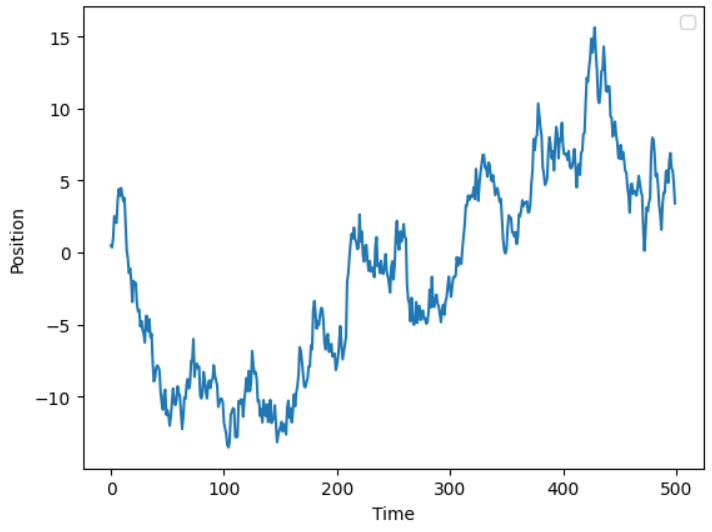
\includegraphics[width=0.5\linewidth]{img/1d-brownian.png}
  \vspace{0.5cm}
  \caption{An illustration of the Wiener process.}
  \label{figure:brownian-motion-illustration}
\end{figure}

\begin{theorem}[Quadratic Variation]
  \label{theorem:quadratic-variation}
  Let $[a, b]$ be an interval in $[0,\infty)$ and partitions
  $$P^n=\{0=t_0^n\le t_1^n\le\ldots\le t_m^n=T\},$$
  with $\left|P^n\right|\to0$ as $n\to\infty$. Then
  \begin{equation}
    \sum\limits_{k=0}^{m_n-1}\left(W\left(t_{k+1}^n\right)-W\left(t_k^n\right)\right)^2\to b-a
  \end{equation}
  as $n\to\infty$.
\end{theorem}

\begin{proof}
  Let $Q_n=\sum\limits_{k=0}^{m_n-1}\left(W\left(t_{k+1}^n\right)-W\left(t_k^n\right)\right)^2$, then
  $$Q_n-(b-a)=\sum\limits_{k=0}^{m_n-1}\left(\left(W\left(t_{k+1}^n\right)-W\left(t_k^n\right)\right)^2-\left(t^n_{k+1}-t^n_k\right)\right).$$

  Hence,
  \begin{align*}
     & \EE[(Q_n-(b-a))^2]                                                                                                                                                                                                                                                                           \\
     & =\sum\limits_{k=0}^{m_n-1}\sum\limits_{j=0}^{m_n-1}\EE  \left[\left(\left(W\left(t_{k+1}^n\right)-W\left(t_k^n\right)\right)^2-\left(t^n_{k+1}-t^n_k\right)\right)\right. \left.\left(\left(W\left(t_{j+1}^n\right)-W\left(t_j^n\right)\right)^2-\left(t^n_{j+1}-t^n_j\right)\right)\right].
  \end{align*}

  If $k\ne j$, due to independent increment, the term becomes the product of two expectations. Since $W(t)-W(s)\sim \N(0,t-s)$ for $t>s\ge 0$, the first expectation is

  $$\EE\left[\left(\left(W\left(t_{k+1}^n\right)-W\left(t_k^n\right)\right)^2-\left(t^n_{k+1}-t^n_k\right)\right)\right]=0.$$

  Therefore, this term vanishes and
  \begin{align*}
    \EE[(Q_n-(b-a))^2]=\sum\limits_{k=0}^{m_n-1}\EE\left[\left(\left(W\left(t_{k+1}^n\right)-W\left(t_k^n\right)\right)^2-\left(t^n_{k+1}-t^n_k\right)\right)^2\right].
  \end{align*}
  Let $Y_k = \dfrac{W\left(t_{k+1}^n\right)-W\left(t_k^n\right)}{\sqrt{t_{k+1}^n-t_k^n}}\sim\N(0,1)$, we have
  \begin{align*}
    \EE\left[\left(\left(W\left(t_{k+1}^n\right)-W\left(t_k^n\right)\right)^2-\left(t^n_{k+1}-t^n_k\right)\right)^2\right] & =\EE\left[(t^n_{k+1}-t^n_k)^2(Y_k^2-1)^2\right]  \\
                                                                                                                           & =(t^n_{k+1}-t^n_k)^2\EE\left[(Y_k^2-1)^2\right].
  \end{align*}
  Let $C=\max\limits_{i=1,\ldots,k}\left\{\EE\left[(Y_k^2-1)^2\right]\right\}$, we have

  $$\EE[(Q_n-(b-a))^2]\le C\sum\limits_{k=0}^{m_n-1}(t^n_{k+1}-t^n_k)^2\to 0 \text{ as } n\to\infty.$$
\end{proof}

Also, every stochastic process is associated with a class of its modifications, whose finite distributions are the same. We say that a stochastic process identifies a \textit{probability law}\index{probability law}. From now on, we denote $P^0$ the probability law of a process starting from time $0$.

\subsection{Markov Processes}

\begin{definition}[Markov Property]
  Let $(\Omega, \F, \PP)$ is a probability space. A stochastic process $\{M_t\}_{t\in[0,T]}$ adapted to a filtration $\{\F_t\}_{t\in[0,T]}$ is a Markov process if
  \begin{equation}
    \EE[M_t|\F_s] = \EE[M_t|M_s],  \forall 0 \le s \le t \le T.
  \end{equation}
  A Markov process is said to be time-homogeneous if $M_t = M_s, a.s.$ for some $t > s$ implies that $M_{t+r} = M_{s+r}, a.s. \forall r\ge0$.
\end{definition}

\begin{definition}[Infinitesimal Generator]
  Let $\{K_t\}$ be a continuous-time semigroup of linear operators on $L^2$. We say that a function $f\in L^2$ belongs to $\mathrm{Dom}(G)$ if the limit
  \begin{equation}
    \lim\limits_{h\downarrow 0}\dfrac{K_hf - K_0f}{h} := Gf
  \end{equation}
  exists in $L^2$. In such cases, $G$ is called the infinitesimal generator of $\{K_t\}$.
\end{definition}

\begin{theorem}[The Derivative of a Function Evolved by a Semi-Group]
  Let $G$ be the generator of a semigroup of linear operators $\{K_t\}$ on $L^2$. For a fixed $f\in\Dom(G)$, set $u(x,t) := (K_tf)(x)$. Then $\partial_t u$ exists for all $t$, and is equal to $Gu$.
\end{theorem}
% \begin{proof}

% \end{proof}

\begin{definition}[Self-space Markov Kernel]
  Let $(\Omega, \F)$ be a measurable space. A function $\kappa: \Omega\times\F\to[0,1]$ is called a (self-space) Markov kernel on $(\Omega, \F)$  if
  \begin{enumerate}[label=(\roman*), ref=(\roman*)]
    \item For any $F\in\F$, the function $\kappa(\cdot, F): \Omega \to [0,1]$ is $\F$-measurable.
    \item For any $\omega\in\Omega$, the function $\kappa(\omega, \cdot): \F\to [0,1]$ is a probability measure on $(\Omega, \F)$.
  \end{enumerate}
\end{definition}

\begin{definition}
  Let $(\Omega, \F)$ be a measurable space. Let $\kappa_1$ and $\kappa_2$ be Markov kernels. The product $\kappa_1\kappa_2 : \Omega \to \F$ is a Markov kernel, defined as
  \begin{equation}
    (\kappa_1\kappa_2)(x,F) = \int_{y\in\Omega}\kappa_2(y,F)\d\kappa_1(x,y).
  \end{equation}
\end{definition}

\begin{definition}[Transition Kernel]
  Let $(\Omega, \F)$ be a measurable space. For every $0\le s\le t\le T$, let $\kappa_{s,t}$ be a Markov kernel on $(\Omega, \F)$. The family $\{\kappa_{s,t}\}$ is called a semigroup of transition kernels if
  \begin{enumerate}[label=(\roman*), ref=(\roman*)]
    \item For any  $t$, $\kappa_{t,t}(x,B) = \delta_{B}(x)$.
    \item For any $0\le r\le s\le t\le T$, $\kappa_{r,t} = \kappa_{r,s}\kappa_{s,t}$.
  \end{enumerate}
\end{definition}

\begin{definition}
  Let $(\Omega, \F)$ be a measurable space and $\{\kappa_{s,t}\}$ is a semigroup of transition kernels. We define $\{K_{s,t}\}$ the semigroup of transition operators on $B(\RR^d,\RR)$ as
  \begin{equation}
    (K_{s,t}f)(x) = \int\limits_{y\in\Omega}f(y)\d \kappa(x,y) := \kappa_{s,t}(f(x)), \forall x\in\RR^d.
  \end{equation}
\end{definition}

\begin{theorem}[Transition Operator Semigroups and Markov Processes]
  Let $X$ be a Markov process with transition kernels $\{\mu_{s,t}\}$, and let $\{K_{s,t}\}$ be the corresponding semigroup of transition operators. Then for any $f \in B(\RR^d, \RR)$, we have
  \begin{equation}
    \label{equation:transition-operator-semigroups-and-markov-process}
    \EE[X_t | \F_s] = (K_{s,t}f)(X_s).
  \end{equation}
  Conversely, let $X$ be any stochastic process, and let $K_{s,t}$ be a semigroup of transition operators such that Equation \ref{equation:transition-operator-semigroups-and-markov-process} is valid (a.s.). Then $X$ is a Markov process.
\end{theorem}
\begin{proof}
  We have
  \begin{align*}
    (K_{s,t}f)(X_s)
     & = \int\limits_{y\in\Omega}f(y)\d \kappa_{s,t}(x,y) \\
     & = \E[f(X_t) | \sigma(X_s)]                         \\
     & = \EE[X_t | \F_s].
  \end{align*}
\end{proof}

\begin{definition}[Martingale Problem]
  Let $G$ be a generator on $\D\subset\C_b(\RR^d, \RR)$. A $d$-dimensional stochastic process $X:=\{X_t\}$ is a solution to the martingale problem for $G$, $\D$, if for any $f\in \D$,
  \begin{equation}
    f(X_t) - \int\limits_0^t Gf(X_s)\d s
  \end{equation}
  is a martingale with respect to ${\F^X_t}$, the natural filtration of X.
\end{definition}

\begin{lemma}
  A stochastic process $X:=\{X_t\}$ is a solution to the martingale problem if and only if
  \begin{equation}
    \EE\left[f(X_t)|\F^X_s\right] - \EE\left[\left.\int\limits_{s}^t Gf(X_r)\d r \right| \F^X_s\right] = f(X_s), \forall 0\le s\le t\le T.
  \end{equation}
\end{lemma}
% \begin{proof}

% \end{proof}

\begin{theorem}
  Let $X$ be a homogeneous Markov process with generator $G$ and cadlag sample paths. Then X solves the martingale problem for $G$, $\C_b(\RR^d, \RR)\cap \mathrm{Dom}(G)$.
\end{theorem}

\begin{definition}
  Let $(\Omega, \F)$ is a probability space. A function $\kappa: \F \times \RR \to [0,1]$ is called a probability kernel.
\end{definition}

\begin{definition}
  Let $\kappa_1$ and $\kappa_2$ be probability kernels. The product of $\kappa_1$ and $\kappa_2$ is defined as
  \begin{equation}
    (\kappa_1\kappa_2)(x, D) = \int\kappa_1(x, D)\d\kappa(x, y).
  \end{equation}
\end{definition}

\begin{definition}
  Let $\D$ be the set of all distributions on $\RR^d$. For every $s,t$, a probability kernel $\kappa_{s,t} : \D \times \D \to [0,1]$ is called a transition kernel if
  \begin{enumerate}[label = (\roman*)]
    \item For all $t\in[0,T]$ and $D\in\D$, $\kappa_{t,t}(D, ) = \mathbf{1}_{D}(\cdot)$.
    \item For any $r\le s\le t$, $\kappa_{r,t}=  \kappa_{r,s}\kappa_{s,t}$.
  \end{enumerate}
  We usually call $\{\kappa_{s,t}\}$ a transition semigroup.
\end{definition}

Each Markov process is associated with a transition semigroup. Conversely, given a transition semigroup, there exists a corresponding Markov process.


\section{Stochastic Integrals}
\label{subsection:stochastic-integrals}
\subsection{Motivation}
Suppose that we want to model the stock price where the time points are in the interval $[0,T]$. We firstly consider a discrete case where $T \in \NN$ and the intermediate time points are $t_n = n, n \in \{0,\ldots, T\}$. Let $p_0$ be the initial stock price at time $t_0$. We wish to establish the formula for the stock price at each time $t_n = n, n \in \{0,\ldots, T\}$ in a nondeterministic way, due to market uncertainty. We can instead formulate the evolution of the price over each time step. Let $\{X_n\}_{n=0}^T$ be a stochastic process where $X_n$ is the price at time $t_n=n$, we have

\begin{equation}
  \begin{cases}
    X_0= p_0 \\
    X_{n+1} - X_n = b(X_n,n) + \sigma(X_n,n)\cdot \texttt{noise}, \,\,\,n\in \{0,\cdots, T-1\},
  \end{cases}
\end{equation}

where $b,\sigma:\RR\times\NN\to\RR$. We select the standard normal random variable for this noise
$$\texttt{noise}:= Z_{n} = W_{n+1}-W_n \sim \N(0,1),$$

by which we hypothesized that if the noise acts more complicatedly, then we can adjust $\sigma(X_n,n)$ to be $\hat{\sigma}(X_n,n)$ such that
$$\sigma(X_n,n)\cdot \texttt{noise} = \hat{\sigma}(X_n,n)(W_{n+1}-W_n) \text{ in } L^2.$$

Our reasonable model is
\begin{equation}
  \label{example:stock-price}
  \begin{cases}
    X_0= p_0 \\
    X_{n+1} - X_n = b(X_n,n) + \sigma(X_n,n)\cdot Z_{n}, \,\,\,n\in \{0,\cdots, T-1\},
  \end{cases}
\end{equation}

\begin{figure}
  \centering
  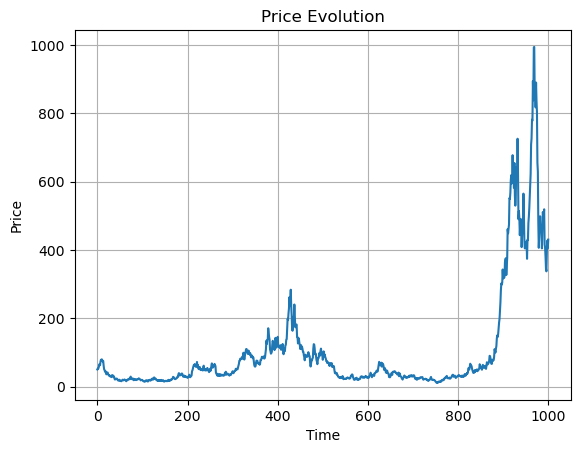
\includegraphics[width=0.7\textwidth]{img/stock-price-sampling.png}
  \vspace{0.25cm}
  \caption[Stock price simulation]{A simulation of stock price evolution by $X_{n+1} - X_n = rX_n + \alpha X_n\cdot Z_{n}$, where $p_0=50, r = 0.005
      \alpha = 0.1$}
\end{figure}

By using time discretization, when it requires to estimate the price at non-integer time, say $t=n+\dfrac{1}{2}$, we need to completely rebuild our model. But intuitively, there must be some change from time $n$ to $n+\dfrac{1}{2}$, then to $n+1$. Itô successfully smoothed the model by Riemann approximation in order to predict the price at any time point in $t\in[0,T]$. Let $P^n[0,T]:=\{0=t^n_0<t^n_1<\ldots<t^n_{m_n}=t\}$ be partitions on $[0,T]$ such that $|P^n|\to 0$ as $n\to\infty$ and write
\begin{align*}
  X(t^n_{k+1})- X(t^n_{k})
   & = b(X(t^n_{k}),t^n_{k})(t^n_{k+1} - t^n_{k+1})+ \sigma(X(t^n_{k}),t^n_{k})(W(t^n_{k+1})-W(t^n_{k})) \\
   & = b(X(t^n_{k}),t^n_{k})\Delta t^n_{k} + \sigma(X(t^n_{k}),t^n_{k})\Delta W(t^n_{k}).
\end{align*}

We have
$$X(t)=X(0)+\sum\limits_{k=0}^{m_n-1}  b(X_k^n,t_k^n)\Delta t^n_{k} + \sum\limits_{k=0}^{m_n-1} \sigma(X(t^n_{k}),t^n_{k})\Delta W(t^n_{k}).$$

Let $(\Omega, \F)$ be a measurable space for the stochastic processes $\{X_t\}_{0\le t\le T}$ and $\{W_t\}_{0\le t\le T}$. Set
$$\hat{b}(\omega, t) :=  b(X_t(\omega),t) \text{ and } \hat{\sigma}(\omega, t) := \sigma(X_t(\omega),t), \forall \omega\in\Omega, t\in[0,T].$$

Then
\begin{equation}
  \label{equation:stochastic-sum}
  X(t,\omega)=X(0,\omega)+\sum\limits_{k=0}^{m_n-1}  \hat{b}(\omega, t_k^n)\Delta t^n_{k} + \sum\limits_{k=0}^{m_n-1} \hat{\sigma}(\omega, t_k^n)\Delta W(t^n_{k}), \forall \omega\in\Omega.
\end{equation}

For each $\omega\in\Omega$, the first sum $\hat{b}(\omega, t_k^n)\Delta t^n_{k}$ converges to the integral $\int\limits_0^T \hat{b}(\omega, t)\d t$, under an assumption that $t\mapsto \hat{b}(\omega, t)$ is Riemann integrable. Therefore, we will try to find the limit of the second sum under appropriate conditions. Note that when we construct such sum, we implicitly assume that $\hat{b}(\omega, t)$ does not depend on $W_s$, for $s\ge t$ i.e. $\hat{b}(\omega, t)$ only depends on the history of the Brownian motion $\{W_t\}$ up to time $t$, not the future of $\{W_t\}$. Let us give a definition for such process.

\begin{definition}[Non-anticipating process]
  Let $W:=\{W_t\}_{t\in[0,T]}$ be a Wiener process, and $\{\W_t\}_{t\in[0,T]}$ be the right-continuous completion of the natural filtration of $W$. Let $\G$ be a $\sigma$-algebra independent of ${\W_t}_{t\in[0,T]}$. Then the non-anticipating filtrations are the ones of the form
  $$\{\sigma(\W_t \cup G)\}_{t\in[0,T]}.$$
  A stochastic process $\{X_t\}_{t\in[0,T]}$ is non-anticipating if it is adapted to some non-anticipating filtration.
\end{definition}

Further conditions are added to guarantee the convergence of $hat{b}(\omega, t_k^n)$, which will be clarified later. In such case, we adapt the usual integration notation as
\begin{equation}
  \sum\limits_{k=0}^{m_n-1} \hat{\sigma}(\omega, t_k^n)\Delta W(t^n_{k}) \xrightarrow{n\to\infty} \int\limits_0^t \hat{\sigma}(\omega, t_k^n)\d W_s = \int\limits_0^t \sigma(X_s,s)\d W_s.
\end{equation}

\subsection{An Example on the Wiener Process}

In Equation \ref{equation:stochastic-sum}. We have selected in initial points $(t_k^n)_{k=1}^{m_n-1}$ in the partition for the limit of the approximations. Unlike the Riemann integral, each point $\tau_k^n = (1-\lambda) t_k^n + \lambda t_{k+1}^n$, where $\lambda\in[0,1]$, for $k=1,\ldots, m_n-1$ results in different a value of the limit
$$\sum\limits_{k=0}^{m_n-1} \hat{\sigma}(\tau_k^n, \omega)\Delta W(\tau^n_{k}).$$

Let us take a ubiquitous example to emphasize this fact.

\begin{example}
  \label{example:wdw}
  Let $P^n[0,T]:=\{0=t^n_0<t^n_1<\ldots<t^n_{m_n}=T\}$ be partitions on $[0,T]$ such that $|P^n|\to0$ when $n\to\infty$ and $\{W_t\}_{t\in[0,T]}$ be real-valued Wiener process. Calculate the limit
  \begin{equation}
    \lim\limits_{n\to\infty}\sum\limits_{k=0}^{m_n-1} W(\tau_k^n)(W(t^n_{k+1})-W(t^n_{k})),
  \end{equation}
  where
  $\tau_k^n = (1-\lambda) t_k^n + \lambda t_{k+1}^n$ for some $\lambda\in[0,1]$.
\end{example}

\begin{solution}
  We have
  \begin{align*}
    R_n
     & = \sum\limits_{k=0}^{m_n-1} W(\tau_k^n)(W(t^n_{k+1})-W({t^n_{k}}))                                                                      \\
     & =
    \sum\limits_{k=0}^{m_n-1}\left[ W(\tau_k^n) - W(t_k^n) + W(t_k^n)\right]\left[W(t^n_{k+1}) - W(\tau_k^n) + W(\tau_k^n) - W(t^n_{k})\right] \\
     & = \underbrace{\sum\limits_{k=0}^{m_n-1}(W(\tau_k^n) - W(t_k^n))(W(t^n_{k+1}) - W(\tau_k^n)) }_{A_n}
    \\
     & \,\,\,\, + \underbrace{\sum\limits_{k=0}^{m_n-1}(W(\tau_k^n) - W(t_k^n))^2  }_{B_n}
    \\
     & \,\,\,\, + \underbrace{ \sum\limits_{k=0}^{m_n-1}(W(t_k^n))(W(t^n_{k+1}) - W(t_k^n))}_{C_n}
  \end{align*}

  Now we study the terms $A_n$, $B_n$ and $C_n$. Let us show that $A_n\to 0$ in $L^2(\Omega)$. Indeed, we have
  \begin{align*}
    \EE[A_n^2]
     & = \EE\left[\left(\sum\limits_{k=0}^{m_n-1}(W(\tau_k^n) - W(t_k^n))(W(t^n_{k+1}) - W(\tau_k^n))\right)^2\right]        \\
     & = \EE\left[\sum\limits_{k=0}^{m_n-1}[(W(\tau_k^n) - W(t_k^n))(W(t^n_{k+1}) - W(\tau_k^n))]^2\right]                   \\
     & \,\,\,\, + \EE\left[\sum\limits_{\substack{k,\ell=0                                                                   \\ k\ne \ell}}^{m_n-1}(W(\tau_k^n) - W(t_k^n))(W(t^n_{k+1}) - W(\tau_k^n))(W(\tau_\ell^n) - W(t_\ell^n))(W(t^n_{\ell+1}) - W(\tau_\ell^n))\right]\\
     & = \sum\limits_{k=0}^{m_n-1}\EE\left[(W(\tau_k^n) - W(t_k^n))^2(W(t^n_{k+1}) - W(\tau_k^n))^2\right]                   \\
     & \,\,\,\, + \sum\limits_{\substack{k,\ell=0                                                                            \\ k\ne \ell}}^{m_n-1}\EE\left[(W(\tau_k^n) - W(t_k^n))(W(t^n_{k+1}) - W(\tau_k^n))(W(\tau_\ell^n) - W(t_\ell^n))(W(t^n_{\ell+1}) - W(\tau_\ell^n))\right]\\
     & = \sum\limits_{k=0}^{m_n-1}\EE\left[(W(\tau_k^n) - W(t_k^n))^2(W(t^n_{k+1}) - W(\tau_k^n))^2\right]                   \\
     & \,\,\,\, + \sum\limits_{\substack{k,\ell=0                                                                            \\ k\ne \ell}}^{m_n-1}\EE\left[(W(\tau_k^n) - W(t_k^n))(W(t^n_{k+1}) - W(\tau_k^n))(W(\tau_\ell^n) - W(t_\ell^n))(W(t^n_{\ell+1}) - W(\tau_\ell^n))\right]\\
     & = \sum\limits_{k=0}^{m_n-1}\EE\left[(W(\tau_k^n) - W(t_k^n))^2\right]  \EE\left[(W(t^n_{k+1}) - W(\tau_k^n))^2\right] \\
     & \,\,\,\, + \sum\limits_{\substack{k,\ell=0                                                                            \\ k\ne \ell}}^{m_n-1}\underbrace{\EE\left[W(\tau_k^n) - W(t_k^n)\right]}_{=0}\EE\left[(W(t^n_{k+1}) - W(\tau_k^n))(W(\tau_\ell^n) - W(t_\ell^n))(W(t^n_{\ell+1}) - W(\tau_\ell^n))\right]\\
     & = \sum\limits_{k=0}^{m_n-1}\EE\left[(W(\tau_k^n) - W(t_k^n))^2\right]  \EE\left[(W(t^n_{k+1}) - W(\tau_k^n))^2\right] \\
     & = \sum\limits_{k=0}^{m_n-1}(1-\lambda)(t_{k+1}^n - t_k)\lambda(t_{k+1}^n - t_k^n)                                     \\
     & \le \lambda(1-\lambda) \sum\limits_{k=0}^{m_n-1}(t_{k+1}^n - t_k)|P^n|                                                \\
     & = \lambda(1-\lambda)T|P^n| \xrightarrow{n\to\infty} 0.
  \end{align*}

  Next, we will show that $B_n\to \lambda T$ in $L^2(\Omega)$.
  \begin{align*}
    \EE[(B_n-\lambda T)^2]
     & = \EE[B_n^2+\lambda^2 T^2 - 2\lambda T B_n]                                                                                                                                            \\
     & = \lambda^2 T^2 - 2\lambda T \EE[ B_n] + \EE[B_n^2]                                                                                                                                    \\
     & = \lambda^2 T^2 - 2\lambda T \sum\limits_{k=0}^{m_n-1} \EE\left[(W(\tau_k^n) - W(t_k^n))^2\right] + \EE\left[\left(\sum\limits_{k=0}^{m_n-1}(W(\tau_k^n) - W(t_k^n))^2\right)^2\right] \\
     & = \lambda^2 T^2 - 2\lambda T \sum\limits_{k=0}^{m_n-1} \lambda (t_{k+1}^n-t_k^n)                                                                                                       \\
     & \,\,\,\, + \sum\limits_{k=0}^{m_n-1}\EE\left[(W(\tau_k^n) - W(t_k^n))^4\right] + \sum\limits_{\substack{k,\ell=0                                                                       \\ k\ne \ell}}^{m_n-1} \EE\left[(W(\tau_k^n) - W(t_k^n))^2(W(\tau_\ell^n) - W(t_\ell^n))^2\right]                                                                                                    \\
     & = -\lambda^2 T^2 + 3\lambda^2\sum\limits_{k=0}^{m_n-1}(t_{k+1}-t_k)^2                                                                                                                  \\
     & \,\,\,\,+ \sum\limits_{\substack{k,\ell=0                                                                                                                                              \\ k\ne \ell}}^{m_n-1} \EE\left[(W(\tau_k^n) - W(t_k^n))^2\right] \EE\left[(W(\tau_\ell^n) - W(t_\ell^n))^2\right] \\
     & = -\lambda^2 T^2 + 3\lambda^2\sum\limits_{k=0}^{m_n-1}(t_{k+1}^n-t_k^n)^2 + \lambda^2\sum\limits_{\substack{k,\ell=0                                                                   \\ k\ne \ell}}^{m_n-1} (t_{k+1}^n-t_k^n)(t_{\ell+1}^n-t_\ell^n) \\
     & = -\lambda^2 T^2 + 2\lambda^2\sum\limits_{k=0}^{m_n-1}(t_{k+1}^n-t_k^n)^2 + \lambda^2\sum\limits_{\substack{k,\ell=0}}^{m_n-1} (t_{k+1}^n-t_k^n)(t_{\ell+1}^n-t_\ell^n)                \\
     & = -\lambda^2 T^2 + 2\lambda^2\sum\limits_{k=0}^{m_n-1}(t_{k+1}^n-t_k^n)^2 + \lambda^2\sum\limits_{\substack{k,\ell=0}}^{m_n-1} (t_{k+1}^n-t_k^n)(t_{\ell+1}^n-t_\ell^n)                \\
     & = 2\lambda^2\sum\limits_{k=0}^{m_n-1}(t_{k+1}^n-t_k^n)^2                                                                                                                               \\
     & \le 2\lambda^2\sum\limits_{k=0}^{m_n-1}|P^n|(t_{k+1}^n-t_k^n)                                                                                                                          \\
     & = 2\lambda^2|P^n|T \xrightarrow{n\to\infty} 0.
  \end{align*}

  The last expression $C_n$ is exactly the case when we choose the initial points.

  Since
  \begin{align*}
    W(t_k^n)(W(t^n_{k+1})-W(t^n_k))
  \end{align*}
  We have
  \begin{align*}
    C_n
     & =\sum\limits_{k=0}^{m_n-1}W(t^n_k)(W(t^n_{k+1})-W(t^n_k))                          \\
     & = \dfrac{1}{2}\left[W^2(t^n_{k+1})-W^2(t^n_k)-(W(t^n_{k+1})-W(^n_k))^2\right]
     & =\dfrac{W^2(T)}{2} -\dfrac{1}{2}\sum\limits_{k=0}^{m_n-1}(W(t^n_{k+1})-W(t^n_k))^2 \\
     & \xrightarrow{n\to\infty} \dfrac{W^2(T)}{2} - \dfrac{T}{2}
  \end{align*}
  Thus,
  $$R_n \xrightarrow{n\to\infty} \dfrac{W^2(T)}{2} + \left(\lambda-\dfrac{1}{2}\right)T.$$
\end{solution}

Two following choices of $\lambda$ are popular in particular
\begin{enumerate}
  \item If $\lambda = 0$, the limit $\lim\limits_{n\to\infty}R_n$ is called an Itô integral, denoted by the conventional integral notation $\int\limits_0^T W\d W$.
  \item If $\lambda = \dfrac{1}{2}$, it is called a Stratonovich integral, denoted by $\int\limits_0^T W\circ\d W$.
\end{enumerate}

In the scope of our project, we concern about the Itô Integral for later applications on stochastic modeling.

\subsection{Construction of the Itô Integral}

Recall that we have adapted the bootstrapping process to construct the Lebesgue integral. In the construction of the Itô Integral, similar strategy is applicable. We define Itô integral for the class of elementary functions, then generalize the result for a function $\hat{\sigma}(\omega, t)$ satisfying some additional conditions. Now we make consistent definitions for such class of functions.

\begin{definition}[Progressively measurable process]
  Let $\{X_t\}_{t\in[0,T]}$ be a stochastic process adapted to a filtration $\{\F_t\}_{t\in[0,T]}$. Then $\{X_t\}_{t\in[0,T]}$ is said to be progressively measurable (progressive) if $X_t$ is $\F_t\otimes\B([0,t])$, for any $t\in[0,T]$.
\end{definition}

\begin{definition}[Elementary process]
  A progressive, non-anticipating process $\{X_t\}_{t\in[0,T]}$ is elementary if there exists a partition
  $$P[0,T]:=\{0=t_0<t_1<\ldots<t^N=T\}$$ such that
  $$X(t) = X(t_n) \text{ if } t \in [t_n, t_{n+1}), \text{ for } j=0,\ldots,N-1.$$
\end{definition}
\begin{remark}
  For an elementary process, the map $t\mapsto X(t,\omega)$ is a step function. We can write an elementary compactly as
  $$X(t) = \sum\limits_{n=0}^{N-1} X(t_n)\mathbf{1}_{[t_n, t_{n+1})}(t),$$
  where $\mathbf{1}$ is the indicator function.
\end{remark}

Denote by $\V := \V[0,T]$ the class of $\L^2$ stochastic processes that are progressively measurable and non-anticipating. We will prove that any process in $\V$ can be approximated by a sequence of elementary process. Throughout the proofs, we will see reasons why a process must be in class $\V$ so that it is Itô integrable.

\begin{definition}
  Let $\{X_t\}_{t\in[0,T]}$ be an elementary process defined on a partition $P[0,T]:=\{0=t_0<t_1<\ldots<t_N=T\}$. The Itô integral of $\{X_t\}_{t\in[0,T]}$ on $[0,t]$ is
  $$\int\limits_0^t X(t)\d W = \sum\limits_{j=0}^{n-1} X(t_j)(W_{j+1}-W_{j}).$$
  If $\int\limits_0^t X(t)\d W < \infty$, the process $\{X_t\}_{t\in[0,T]}$ is said to be Itô-integrable.
\end{definition}

\begin{lemma}[Approximation of a bounded, continuous process by elementary processes]
  \label{lemma:approximation-1}
  Let $X:=\{X_t\}_{t\in[0,\infty]}$ be a stochastic process that is continuous, progressive, non-anticipating and bounded on $[0, T]$. Then there exists a sequence $(X_n)_{n\in\NN} := (\{X_n(t)\}_{t\in[0,\infty]})_{n\in\NN}$ of bounded, Itô-integrable elementary processes such that
  $$X_n \xrightarrow{n\to\infty} X \text{ in } \L^2.$$
\end{lemma}

\begin{proof}
  Set
  \begin{equation}
    X_n(t) := \sum\limits_{i=1}^\infty X\left(i/2^n\right) \1_{[i/2^n, (i+1)/2^n)}(t).
  \end{equation}
  This is clearly elementary, bounded and square-integrable on $[0, T]$. For any fix $\omega$, since $X(t,\omega)$ is continuous, we have
  $$\lim\limits_{n\to\infty}\int\limits_0^T (X(t,\omega) - X_n(t,\omega))^2 \d t = 0.$$

  By dominated convergence,

  \begin{align*}
    \lim\limits_{n\to\infty}\|X(t) - X_n(t)\|_{\L^2}
     & = \lim\limits_{n\to\infty}\int_\Omega\int\limits_0^T (X(t,\omega) - X_n(t,\omega))^2 \d t \d P \\
     & = \int_\Omega\int\limits_0^T \lim\limits_{n\to\infty}(X(t,\omega) - X_n(t,\omega))^2 \d t \d P \\
     & = 0.
  \end{align*}
\end{proof}

\begin{lemma}[Approximation of a bounded process by bounded, continuous processes]
  \label{lemma:approximation-2}
  Let $X$ be a stochastic process that is progressive, non-anticipating, bounded on $[0, T]$. Then there exists a sequence $(X_n)_{n\in\NN}$ of continuous, progressive, non-anticipating and bounded on $[0, T]$ processes such that
  $$X_n \xrightarrow{n\to\infty} X \text{ in } \L^2.$$
\end{lemma}
\begin{proof}
  Let $M$ be the bound on the norm of X. For each $n$, pick a probability density $f_n(t):\RR\to\RR$ support is the interval $(-1/n, 0)$. Set
  $$X_n(t) := \int\limits_0^t f_n(s-t) X(s) \d s.$$
  Then $X_n$ is continuous, bounded, progressively measurable, and non-anticipating. Therefore, for any fix $\omega$, we
  $$\int\limits_0^T (X(t,\omega) - X_n(t,\omega))^2 \d t \xrightarrow{n\to\infty} 0.$$
  Convergence in $\L^2$ follows from dominated convergence.
\end{proof}


\begin{lemma}[Approximation of a $\V$ process by bounded processes]
  \label{lemma:approximation-3}
  Let $X$ be an $\L^2$ stochastic process that is progressive, non-anticipating. Then there exists a sequence $(X_n)_{n\in\NN}$ of progressive, non-anticipating and bounded on $[0, T]$ processes such that
  $$X_n \xrightarrow{n\to\infty} X \text{ in } \L^2.$$
\end{lemma}
\begin{proof}
  Set $X_n(t) = (-n \vee X(t)) \wedge n$. Then $X_n$ is bounded. The result follows from dominated convergence.
\end{proof}

\begin{theorem}[Approximation of a $\V$ process by elementary processes]
  Let $X$ be an $\L^2$ stochastic process that is progressive, non-anticipating. Then there exists a sequence $(X_n)_{n\in\NN}$ of bounded, Itô-integrable elementary processes such that
  $$X_n \xrightarrow{n\to\infty} X \text{ in } \L^2.$$
\end{theorem}
\begin{proof}
  The result follows by Lemmas \ref{lemma:approximation-1}, \ref{lemma:approximation-2} and \ref{lemma:approximation-3}.
\end{proof}

\begin{lemma}[Itô isometry for elementary processes]
  \label{lemma:ito-isometry-for-elementary-process}
  Let $\{X_t\}_{t\in[0,T]}$ be a elementary process. Then
  $$\EE\left[\left(\int\limits_0^T X\d W\right)^2\right] = \EE\left[\int\limits_0^T X^2\d t\right] = \|X\|_{\L^2}.$$
\end{lemma}


\begin{proof}
  Let $R_n=\sum\limits_{k=0}^{m_n-1} X(t_k^n)\Delta W(t^n_{k})$. We have
  \begin{align*}
    \EE\left[R_n^2\right]
     & = \EE\left[\sum\limits_{k,\ell = 0}^{m_n-1}X(t_k^n)X(t_\ell^n)\Delta W(t^n_{k}) \Delta W(t^n_{\ell})\right] \\
     & = \sum\limits_{k,\ell = 0}^{m_n-1}\EE\left[X(t_k^n)X(t_\ell^n)\Delta W(t^n_{k}) \Delta W(t^n_{\ell})\right]
  \end{align*}
  If $k \ne \ell$, then $\Delta W(t^n_{k})$ and $\Delta W(t^n_{\ell})$ are independent. Hence,
  \begin{align*}
    \EE\left[X(t_k^n)X(t_\ell^n)\Delta W(t^n_{k}) \Delta W(t^n_{\ell})\right]
     & = \EE\left[X(t_k^n)X(t_\ell^n)\Delta W(t^n_{k})\right]\EE\left[\Delta W(t^n_{\ell})\right] \\
     & =0.
  \end{align*}

  If $k = \ell$, then
  \begin{align*}
    \EE\left[X(t_k^n)X(t_\ell^n)\Delta W(t^n_{k}) \Delta W(t^n_{\ell})\right]
     & =\EE\left[X^2(t_k^n)\right] \EE\left[\Delta W(t^n_{k})^2\right] \\
     & = \EE\left[X^2(t_k^n)\right] (t_{k+1}^n-t_k^n).
  \end{align*}
  Therefore,
  \begin{align*}
    \EE\left[R_n^2\right]
     & =\sum\limits_{k}^{m_n-1} \EE\left[X^2(t_k^n)\right] (t_{k+1}^n-t_k^n)
  \end{align*}
  Taking the limits when $n\to\infty$, we complete the proof.
\end{proof}

\begin{theorem}[Itô integrals of Approximating Elementary Processes Converge]
  Let $(X_n)_{n\in\NN}$ be a sequence of $\V$ elementary processes converging to $X$ in $\L^2$. Then the sequence
  $$R_n(X) = \lim\limits_{n\to\infty}\int\limits_0^T X_n\d W$$
  converges in $L^2$. Moreover, this limit is the same for any such approximating sequence $(X_n)$.
\end{theorem}

\begin{proof}
  Since $\L^2$ is Banach and $(X_n)$ converges, $(X_n)$ is Cauchy. Hence, for any $\epsilon>0$, there exists $N\in\NN$ such that
  $$\|X_{n+N} - X_{N}\|\le\epsilon.$$
  Since $X_{n+N}$ and $X_{N}$ are elementary, so is their difference. By Lemma \ref{lemma:ito-isometry-for-elementary-process},
  $$\EE\left[\left(\int\limits_a^b (X_{n+N}-X_n)\d W \right)^2\right] < \epsilon^2.$$
  Therefore, $(R_n)$ is Cauchy in $L^2$. Since $L^2$ is Banach, $(R_n)$ has a limit. If there exists another approximating elementary sequence $(Y_n)$, then their Itô integral sequence $(S_n)$ is also Cauchy. On the other hand, for any $\epsilon >0$, there exist $m,n\in\NN$ such that
  $$\|X_m-Y_n\| \le \|X_m-X\| + \|Y_n - X\|\le \epsilon.$$
  Hence, the limits of their Itô integral must be equal.
\end{proof}

\begin{definition}
  Let $X\in \V$. The Itô integral of $X$ is defined by
  \begin{equation}
    \int\limits_0^T X\d W =  \lim\limits_{n\to\infty}\int\limits_0^T X_n\d W,
  \end{equation}
  where $(\{X_n(t)\}_{t\in[0,T]})_{n\in\NN}$ is a sequence of elementary functions such that
  $$X_n \xrightarrow{n\to\infty} X \text{ in } \L^2.$$
\end{definition}

\begin{theorem}[Properties of Itô integral]
  \label{theorem:prop}
  For all constants $a,b\in\RR$ and $\sigma,H\in\mathcal{V}(S,T)$, we have
  \begin{enumerate}
    \item Linearity: $\int\limits_{S}^T(aG+bH)\d W = a\int\limits_{S}^TG\d W+b\int\limits_{S}^TH\d W$.
    \item $\EE\left[\int\limits_{S}^TG\d W\right]=0$.
    \item Itô isometry: $\EE\left[\left(\int\limits_{S}^TG\d W\right)^2\right]=\EE\left[\int\limits_{S}^TG^2\d t\right]$.
    \item $\EE\left[\int\limits_{S}^TG\d W\int\limits_{S}^TH\d W\right]=\EE\left[\int\limits_{S}^TGH\d W\right]$.
  \end{enumerate}
\end{theorem}

With the linearity property, we are able to define multidimensional Itô integral.

\begin{definition}
  Let $\sigma=(G_{ij})$, where $G_{ij}, 1\le i\le n, 1\le j\le m$ be real-valued stochastic processes. Also, $W=(W_j)$, where $W_j,1\le j\le m$ be real-valued Wiener process. Then for some $T\ge S\ge 0$
  \begin{equation}
    \int\limits_S^T \sigma\d W=\int\limits_S^T\begin{pmatrix}
      G_{11} & \cdots & G_{1m} \\
      \vdots & \ddots & \vdots \\
      G_{n1} & \cdots & G_{nm}
    \end{pmatrix}\begin{pmatrix}
      \d W_1 \\\vdots\\\d W_m
    \end{pmatrix}
  \end{equation}
  is an $n$-dimensional vector whose $i$th column is the sum of $m$ one-dimensional integrals
  $$\sum\limits_{j=1}^m \int\limits_S^T G_{ij}\d W_k.$$
\end{definition}

\subsection{Itô's Formulas}
Similarly to ordinary differential equations, there are the chain rule and the product rule in SDE calculus.
\begin{theorem}[One-dimensional Itô's chain rule]
  Suppose that $X_t$ has the stochastic differential
  $$\d X = u\d t + v\d W_t.$$
  Let $g\in C^2(\RR\times[0,\infty))$. Then
  $$Y_t=g(X_t,t)$$
  is given by
  \begin{equation}
    \label{equation:1dchainrule}
    \d Y_t=\dfrac{\partial g}{\partial t}(X_t,t)\d t+\dfrac{\partial g}{\partial x}(X_t,t)\d X_t+\dfrac{1}{2}\dfrac{\partial^2 g}{\partial x^2}(X_t,t)\cdot(\d X_t)^2,
  \end{equation}
  where $(\d X_t)^2=(\d X_t)\cdot(\d X_t)$ is computed according to the rules
  $$\d t\cdot\d t = \d t\cdot\d W_t = \d W_t\cdot\d t = 0, \d W_t\cdot\d W_t=\d t.$$
\end{theorem}

\begin{theorem}[One-dimensional Itô's product rule]
  Suppose $\{X_1(t)\}_{[0,T]}$ and $\{X_2(t)\}_{[0,T]}$ satisfy the following SDEs
  $$\begin{cases}
      \d X_1 = b_1\d t+\sigma_1\d W \\
      \d X_2 = b_2\d t+\sigma_2\d W
    \end{cases}(0\le t\le T).$$
  Then
  \begin{equation}
    \label{theorem:ito-product}
    \d (X_1X_2)=X_2\d X_1+X_1\d X_2+\sigma_1\sigma_2\d t
  \end{equation}
\end{theorem}

% \begin{theorem}[Multidimensional Itô's chain rule]
% \label{equation:mdchainrule}
% \end{theorem}


\subsection{Properties of the Itô Process}

\begin{definition}
  Let $b$ be a non-anticipating measurable process, $\sigma$ be Itô-integrable, and $X_0$ be an $L^2$ random variable independent of $W$. Then the integral
  $$X_t := X_0 + \int_0^t b(s) \d s + \int_0^t \sigma(s) dW$$
  is called an Itô process.
\end{definition}

% \begin{theorem}
%   \label{every-ito-process-is-non-anticipating}
%   Every Itô process is non-anticipating.
% \end{theorem}
\section{Stochastic Differential Equations}
Stochastic differential equations (SDEs) plays a major role in continuous-time diffusion models beginning from Anderson's theorem on reverse-time diffusion \cite{anderson1982reverse}. This section develops related backgrounds to prove this theorem.

\subsection{Introduction and Definition of an SDE}

In Section \ref{subsection:stochastic-integrals}, we see that without  a stochastic term $\int\limits_0^t \sigma(X_s,s)\d W_s$, our model become an ordinary deterministic integral
\begin{equation}
  \label{equation:ordinary-integral}
  \begin{cases}
    X_t - X_0 = \int\limits_0^t b(X_s,s)\d s \\
    X_0 = p_0.
  \end{cases}
\end{equation}

We know that such integral is associated with an ordinary differential equation (ODE)
\begin{equation}
  \label{equation:ode}
  \begin{cases}
    \d X_t = b(X_t,t) \\
    X_0 = p_0.
  \end{cases}
\end{equation}

The ODE \ref{equation:ode}, in which $b(X_t,t)$ depends on the time $t$, is called non-autonomous. We can convert this ODE into an autonomous form.

\begin{equation}
  \label{equation:autonomous-ode}
  \begin{cases}
    \d \begin{bmatrix}
         X_t \\ y_t
       \end{bmatrix} = \begin{bmatrix}
                         b(X_t,y_t) \\ 1
                       \end{bmatrix} \\
    \begin{bmatrix}\d t
      X_0 \\ y_0
    \end{bmatrix} = \begin{bmatrix}
                      p_0 \\ 0
                    \end{bmatrix}
  \end{cases}
\end{equation}

In the same sense, a stochastic differential equation presents a differential form of a stochastic integral, given in the following definition.

\begin{definition}
  Let $\{X(t)\}_{t\in[0,T]}$ be a $d_X$-dimensional stochastic process. Suppose that there is a function $b:\RR^{d_X}\times [0,T]\to\RR^{d_X}$ that is $(\B(\RR^{d_X})\otimes \B([0,T)),\B(\RR^{d_X}))$-measurable, and there is a function $\sigma:\RR^{d_X}\times [0,T]\to\RR^{d_X\times d_W}$ that is $(\B(\RR^{d_X})\otimes \B([0,T)), \B(\RR^{d_X\times d_W}))$-measurable, such that
  $$X(s) = X(0)+\int\limits_{0}^s b(X_t,t)\d t + \int\limits_{0}^s \sigma(X_t,t)\d W, \forall 0\le s \le T,$$
  where $W = W(t)$ is a $d_W$-dimensional Wiener process. We say that $\{X(t)\}_{t\in[0,T]}$ is a solution to the non-autonomous stochastic differential equation
  \begin{equation}
    \label{definition:sde}
    \begin{cases}
      \d X_t & = b(X_t,t)\d t+\sigma(X_t,t)\d W \\
      X_{0}  & = Z.
    \end{cases}
  \end{equation}
\end{definition}

Similarly to ODEs, we can convert \ref{definition:sde} into an autonomous form
\begin{equation}
  \label{equation:autonomous-sde-convert}
  \begin{cases}
    \d \begin{bmatrix}
         X_t \\ y_t
       \end{bmatrix} & =
    \begin{bmatrix}
      b(X_t,y_t) \\ 1
    \end{bmatrix}
    \d t + \begin{bmatrix}
             \sigma(X_n,t) \\ 0
           \end{bmatrix}\d W            \\
    \begin{bmatrix}
      X_{0} \\ y_{0}
    \end{bmatrix}    & = \begin{bmatrix}
                           Z \\ 0
                         \end{bmatrix}.
  \end{cases}
\end{equation}
Therefore, we will later study autonomous SDEs of the form
\begin{equation}
  \label{definition:autonomous-sde}
  \begin{cases}
    \d X_t & = b(X_t)\d t+\sigma(X_t)\d W \\
    X_{0}  & = Z.
  \end{cases}
\end{equation}

\begin{example}
  \begin{enumerate}
    \item []
    \item The \textit{geometric Brownian motion}
          $$\d X_t = b_0X_t\d t +  \sigma_0 X_t\d W_t$$
          is used in financial mathematics as an equation for the dynamics of a stock price \cite{reddy2016simulating}.
    \item The equation
          $$\d X_t=\sqrt{\beta(t)}\d W$$
          is used in the continuous-time setting of Denoising Diffusion Probabilistic Models \cite{ho2020denoising}.
  \end{enumerate}
\end{example}

Given an SDE \ref{definition:sde}, we can sample some $X_t$, where $t\in[0,T]$ using discretization. Let $\Delta t$ be the time step. For $0<t<T$, set $N=\dfrac{T}{\Delta t}$ and compute
$$X_{n+1} = X_n + b(X_n, n\Delta t)\Delta t + \sigma(X_n, n\Delta t)\sqrt{\Delta t} Z_n, n = 1,2 \ldots, N-1,$$
where $Z_1,Z_2,\ldots, Z_n\sim\N(0,I)$.

\subsection{Solutions to an SDE}


\begin{definition}[Maximum process]
  Let $\{X_t\}_{t\in[0,T]}$ be a real-valued stochastic process. The maximum process $\{X^*_t\}_{t\in[0,T]}$ is defined as
  $$X^*_t = \sup\limits_{0\le s\le t} |X_s|$$
\end{definition}

\begin{definition}[The Space $\Q\M(T)$]
  Let $\Q\M(T)$, where $T>0$ be the space of all non-anticipating, real-valued and square-integrable processes $\{X_t\}_{t\in[0,T]}$.
\end{definition}

\begin{proposition}
  The function $\|\cdot\|_{\Q\M(T)}:\Q\M(T)\to\RR$ defined by
  $$\|X\|_{\Q\M(T)} = \|X^*_T\|_{L^2(\Omega)},\forall X\in \Q\M(T)$$
  is a norm on $\Q\M(T)$. Moreover, the normed space $\left(\Q\M(T),\|\cdot\|_{\Q\M(T)}\right)$ is Banach.
\end{proposition}

\begin{definition}[Picard operator]
  Consider the SDE \ref{definition:autonomous-sde}. The corresponding integral operator $P_{X_0,b,\sigma}$ for an Itô process $Y:=\{Y_t\}_{t\in[0,T]}$ is defined as
  \begin{equation}
    \label{equation:picard-operator}
    P_{X_0,b,\sigma} Y_t = X_0 + \int\limits_0^t b(Y_s)\d s + \int\limits_0^t \sigma(Y_s)\d W.
  \end{equation}
  We also define $P_{X_0,b,\sigma} Y := \{P_{X_0,b,\sigma} Y_t\}_{t\in[0,T]}$.
\end{definition}

\begin{lemma}
  \label{lemma:inequality-for-Piscard-operator-and-QM-norm}
  Let $b:\RR\to\RR$ and $\sigma:\RR\to\RR$ be uniformly Lipschitz continuous functions, and abbreviate $P_{X_0,b,\sigma}$ by $P$. Let $X$ and $Y$ be one-dimensional Itô processes defined by $b$ and $\sigma$. Then there exists a constant $D\in\RR$ such that
  \begin{equation}
    \|PX - PY\|_{\Q\M(t)}^2 \le D\int\limits_0^t\|X-Y\|_{\Q\M(s)}^2\d s, t\in[0,T]
  \end{equation}
\end{lemma}

\begin{proof}
  For each $t\in[0,T]$ and $\omega\in\Omega$, we have
  \begin{align*}
    \left|PX_t(\omega)-PY_t(\omega)\right|
     & = \left|\int\limits_0^t (b(X_s(\omega))-b(Y_s(\omega)))\d s + \int\limits_0^t (\sigma(X_s(\omega))-\sigma(Y_s(\omega)))\d W\right|                                                 \\
     & \le \left|\int\limits_0^t (b(X_s(\omega))-b(Y_s(\omega)))\d s\right| + \left|\int\limits_0^t (\sigma(X_s(\omega))-\sigma(Y_s(\omega)))\d W\right|                                  \\
     & \le \int\limits_0^t K_b|X_s(\omega)-Y_s(\omega)|\d s + \int\limits_0^t K_\sigma|X_s(\omega)-Y_s(\omega)|\d W                                      & \text{ (Lipschitz continuity)} \\
  \end{align*}
  Hence
  \begin{align*}
    \sup\limits_{0\le r\le t}\left|PX_t(\omega)-PY_t(\omega)\right|
     & \le \sup\limits_{0\le r\le t}\left(\int\limits_0^r K_b|X_s(\omega)-Y_s(\omega)|\d s + \int\limits_0^r K_\sigma|X_s(\omega)-Y_s(\omega)|\d W\right) \\
     & \le \int\limits_0^t K_b|X_s(\omega)-Y_s(\omega)|\d s + \int\limits_0^t K_\sigma|X_s(\omega)-Y_s(\omega)|\d W
  \end{align*}
  Therefore,
  \begin{align*}
    \left\|PX-PY\right\|_{\Q\M(t)}^2
     & \le \EE\left[\left(\sup\limits_{0\le r\le t}\left(PX_t-PY_t\right)^2\right)\right]                                                                           \\
     & \le  \EE\left[\left(\int\limits_0^t K_b|X_s-Y_s|\d s + \int\limits_0^t K_\sigma|X_s-Y_s|\d W\right)^2\right]                                                 \\
     & \le \dfrac{1}{2}\EE\left[\left(\int\limits_0^t K_b|X_s-Y_s|\d s\right)^2+\left(\int\limits_0^t K_\sigma|X_s-Y_s|\d W\right)^2\right]                         \\
     & \le \dfrac{1}{2}\EE\left[K_b t\int\limits_0^t (X_s-Y_s)^2\d s+K_\sigma\left(\int\limits_0^t |X_s-Y_s|\d W\right)^2\right]
     & \text{(Jensen inequality)}                                                                                                                                   \\
     & \le 2\EE\left[K_b^2 t\int\limits_0^t (X_s-Y_s)^2\d s+K_\sigma^2\int\limits_0^t (X_s-Y_s)^2\d s\right]                                & \text{(Itô isometry)} \\
     & = 2(K_b^2 t+K_\sigma^2)\EE\left[\int\limits_0^t (X_s-Y_s)^2\d s\right]                                                                                       \\
     & \le 2t(K_b^2 t+K_\sigma^2)\int\limits_0^t \|X_s-Y_s\|^2_{\Q\M(s)}\d s                                                                                        \\
     & \le 2T(K_b^2 T+K_\sigma^2)\int\limits_0^t \|X_s-Y_s\|^2_{\Q\M(s)}\d s                                                                                        \\
     & = D\int\limits_0^t \|X_s-Y_s\|^2_{\Q\M(s)}\d s.
  \end{align*}
  The proof is completed.
\end{proof}

\begin{theorem}[Existence and uniquness of solutions to SDEs in one dimension]
  \label{theorem:existence-and-uniqueness-solution-to-sdes-in-one-dimension}
  Let there be the autonomous one-dimensional SDE
  \begin{equation}
  \label{equation:autonomous-one-dimensional-sde}
    \begin{cases}
      \d X_t = b(X_t)\d t+\sigma(X_t)\d W \\
      X_{0} = Z.
    \end{cases}
  \end{equation}
  If $b:\RR\to\RR$ and $\sigma:\RR\to\RR$ are uniformly Lipschitz continuous, then there exists a square-integrable, real-valued Itô process $\{X_t\}_{t\in[0,T]}$ that solves Equation \ref{equation:autonomous-one-dimensional-sde}. Moreover, this solution is unique almost surely.
\end{theorem}

\begin{proof}
  We begin by proving the existence of $X$, along with that $X\in\L^2$. Let us abbreviate the Picard operator $P_{X_0,b,\sigma}$ by $P$. For each $t\in[0,T]$, set
  \begin{align*}
    X_0(t)  & = X_0   \\
    X_{n+1} & = PX_n.
  \end{align*}
  We will show that $\{X_n\}$ is Cauchy in $\Q\M(T)$. For $n\in\NN_0$, let
  \begin{equation}
    \phi_n(t) := \|X_{n+1}-X_n\|^2_{\Q\M(T)}.
  \end{equation}
  Because of the supremum embedded in the $\Q\M(T)$-norm, $\phi_n$ is non-decreasing for each $n\in\NN$. Using Lemma \ref{lemma:inequality-for-Piscard-operator-and-QM-norm}, for each $n\in\NN$, we have
  \begin{align*}
    \phi_n(t)
     & = \|PX_{n}-PX_{n-1}\|^2_{\Q\M(T)}                     \\
     & \le D\int\limits_0^t\|X_{n}-X_{n-1}\|_{\Q\M(s)}^2\d s \\
     & = D\int\limits_0^t\phi_{n-1}(s)\d s                   \\
  \end{align*}
  On the other hand, note that $b(X_0) \le \sup\limits_{\omega\in\Omega}|X_0| + b(0) := A$, and similarly, $\sigma(X_0)\le B$, for some constant $B$, since $X_0\in L^2$, we have
  \begin{align*}
    \phi_0(t)
     & = \|X_1-X_0\|^2_{\Q\M(T)}                                                                   \\
     & \le \EE\left[\left(\int_0^tb(X_0)\d s + \int_0^t\sigma(X_0)\d W\right)^2\right]             \\
     & \le \EE\left[\left(\int_0^tA\d s + \int_0^tB\d W\right)^2\right]                            \\
     & \le 2\left[\EE\left[\left(\int_0^tA\d s\right)^2+\left(\int_0^tB\d W\right)^2\right]\right] \\
     & = 2\left[\EE\left[A^2t^2+\int_0^tB^2\d s\right]\right]                                      \\
     & = 2(A^2t^2+B^2t)                                                                            \\
     & \le 2(A^2T+B^2)t                                                                            \\
     & = Ct.
  \end{align*}
  Using induction, there exists a constant $C_1$ such that
  $$  \phi_n(t) \le \dfrac{C_1t^{n+1}}{(n+1)!}\xrightarrow{n\to\infty}0 \text{ in } \Q\M(t).$$
  Therefore, there exists the limit
  $$X(t)=\lim\limits_{n\to\infty}X_n(t)\in\Q\M(t).$$
  To show that $X$ is a solution to \ref{equation:autonomous-one-dimensional-sde}, we have to point out that $PX=X$. This is true because $PX$ is also the limit of $(X_n)$
  \begin{align*}
    \|PX-X_{n+1}\|_{\Q\M(t)}
     & =  \|PX-PX_{n}\|_{\Q\M(t)}                      \\
     & = DT \|X-X_n\|_{\Q\M(t)}                        \\
     & \xrightarrow{n\to\infty} 0 \text{ in } \Q\M(t).
  \end{align*}

  To prove uniqueness, suppose that there is another solution $Y$, then $PY=Y$. We have
  \begin{align*}
    \|X-Y\|_{\Q\M(t)}^2
     & \le \|PX-PY\|_{\Q\M(t)}^2            \\
     & \le D\int_0^t\|X-Y\|_{\Q\M(s)}^2\d s \\
  \end{align*}
  By Lemma \ref{lemma:gronwall-inequality}, we have $\|X-Y\|_{\Q\M(t)}^2\le0$, implying that $X_t = Y_T a.s.$
\end{proof}

\begin{theorem}[Existence and uniquness of solutions to SDEs in multidimension]
  \label{theorem:existence-and-uniqueness-solution-to-sdes-in-multidimension}
  Let there be the autonomous one-dimensional SDE \label{equation:autonomous-multidimensional-sde}
  $$\begin{cases}
      \d X_t = b(X_t)\d t+\sigma(X_t)\d W \\
      X_{0} = Z
    \end{cases}.$$
  If $b$ and $\sigma$ are uniformly Lipschitz continuous in the norm $\|\cdot\|_2$. Then there exists a square-integrable, non-anticipating real-valued stochastic process $X := \{X_t\}_{t\in[0,T]}$ that solves Equation \ref{equation:autonomous-multidimensional-sde}. Moreover, this solution is unique almost surely.
\end{theorem}

\begin{proof}
  Each element $X_t^{(k)}$ of $X_t=\left(X_t^{(1)}, \ldots, X_t^{(d_X)}\right)$ always solves the corresponding elemental SDE
  \begin{align*}
    \d X_t^{(k)} = b^{(k)}(X_t)\d t + \left(\sum\limits_{j=1}^{d_W} \sigma^{(kj)}(X_t)\right)\d W^{(k)},
  \end{align*}
  for any other $X_\ell, \ell\ne k$. Hence, there exists a solution $X$. The argument for uniqueness is similar to the case of one-dimensional SDEs.
\end{proof}

% \begin{theorem}[Solution to an SDE is Strongly Markov]
%   \label{theorem:solution-to-an-sde-is-strongly-markov}

% \end{theorem}

\subsection{Kolmogorov's Equations}
% Since a solution $\{X_t\}_{[t_0,T]}$ to Equation \ref{definition:sde} is a stochastic process, it is possible to define the transition probability
% $$\PP(X_t\in A | X_s = y) = \int\limits_{A} p(x,t | y,s)\d x,$$
% where $p(x,t | y,s)\d x := \PP(X_t\in [x,x+\d x) | X_s = y)$. Specifically, $p(x,t | y,t) = \delta_0(\{x-y\})$.

\begin{definition}
  Let $\{X_t\}$ be a time-homogeneous Itô diffusion in $\RR^d$. Denote $\EE^x[X_t] := \EE[X_t|X_0=x]$ and define
  \begin{equation}
    \label{equation:generator}
    Gf(x) = \lim\limits_{t\downarrow 0}\dfrac{\EE^x[f(X_t)]- f(x)}{t}, x\in\RR^d,
  \end{equation}
  If the limit in Equation \ref{equation:generator} exists, then $G$ is called the generator of the process $\{X_t\}$ with respect to the function $f:\RR^d\to \RR$. The set of all functions $f$ such that the limit exists for any $x\in\RR^d$ is denoted by $\mathrm{Dom}(G)$.
\end{definition}

\begin{lemma}
  \label{lemma:generator}
  Let $\{Y_t\}$ be a $d_Y$-dimensional Itô diffusion and $\{W_t\}$ be a $d_W$-dimensional Wiener process, such that
  $$Y_t := Y^{x}_t = x + \int\limits_0^t b(\omega, s) \d s + \int\limits_0^t \sigma(\omega, s) \d W.$$
  Let $f:\RR^d\to \RR$ be twice differentiable and have a compact support. Then
  \begin{equation}
    \EE^x[f(Y_t)] = f(x) + \EE^x\left[\int\limits_0^t\left(\sum\limits_{i=1}^{d_Y} b_i(\omega,s)\dfrac{\partial f}{\partial x_i}(Y_s) + \dfrac{1}{2}\sum\limits_{i,j=1}^{d_Y} \sigma\sigma^\top (\omega, s)\dfrac{\partial^2f}{\partial x_i \partial x_j}(Y_s)\right)\d s \right].
  \end{equation}
\end{lemma}
\begin{proof}
  Let $Z = f(Y)$. According to Itô formula, we have
  \begin{align*}
    \d Z
     & = \sum\limits_{i=1}^{d_Y}\dfrac{\partial f}{\partial x_i}(Y)\d Y_i + \dfrac{1}{2}\sum\limits_{i,j=1}^{d_Y} \dfrac{\partial^2f}{\partial x_i \partial x_j}(Y)\d Y_i \d Y_j                                                                               \\
     & = \sum\limits_{i=1}^{d_Y} b_i \dfrac{\partial f}{\partial x_i}\d t + \dfrac{1}{2}\sum\limits_{i,j=1}^{d_Y} \dfrac{\partial^2f}{\partial x_i \partial x_j}(v\d W)_i (v\d W)_j +  \sum\limits_{i=1}^{d_Y}\dfrac{\partial f}{\partial x_i}(\sigma \d W)_i.
  \end{align*}
  Also,
  \begin{align*}
    (v\d W)_i (v\d W)_j
     & = \left(\sum\limits_{k=1}^{d_W}\sigma_{ik}\d W_k\right)\left(\sum\limits_{\ell=1}^{d_W}\sigma_{j\ell}\d W_\ell\right) \\
     & = \left(\sum\limits_{k=1}^{d_W}\sigma_{ik}\sigma_{jk}\right)\d t                                                      \\
     & = (\sigma\sigma^\top)_{ij}\d t.
  \end{align*}
  Therefore,
  \begin{align*}
    f(Y_t)
    = f(Y_0) + \int\limits_0^t\left(\sum\limits_{i=1}^{d_Y}b_i\dfrac{\partial f}{\partial x_i} + \dfrac{1}{2}\sum\limits_{i,j=1}^{d_Y} (\sigma\sigma^\top)_{ij} \dfrac{\partial^2f}{\partial x_i \partial x_j}\right) \d s +  \sum\limits_{i=1}^{d_Y}\sum\limits_{j=1}^{d_W}\int\limits_0^t\sigma_{ij}\dfrac{\partial f}{\partial x_i} \d W_j.
  \end{align*}
  We finally take the expectations of two sides to complete the proof.
\end{proof}

\begin{theorem}
  \label{theorem:generator}
  Let $\{X_t\}$ be an Itô diffusion satisfying
  $$\d X_t = b(X_t)\d t + \sigma(X_t)\d W.$$
  If $f:\RR^d\to \RR$ is bounded and twice differentiable, then
  \begin{equation}
    Gf(x) = \sum\limits_{i=1}^{d_Y} b_i \dfrac{\partial f}{\partial x_i} + \dfrac{1}{2}\sum\limits_{i,j=1}^{d_Y} (\sigma\sigma^\top)_{ij}\dfrac{\partial^2f}{\partial x_i \partial x_j}.
  \end{equation}
\end{theorem}
\begin{proof}
  The proof is derived using Lemma \ref{lemma:generator} and that $\{X_t\}$ is Markovian.
\end{proof}

\begin{theorem}[Kolmogorov Forward Equation]
  Let $X$ be an Itô diffusion with generator
  $$ Gf(x) = \sum\limits_{i=1}^{d_Y} b_i \dfrac{\partial f}{\partial x_i} + \dfrac{1}{2}\sum\limits_{i,j=1}^{d_Y} (\sigma\sigma^\top)_{ij}\dfrac{\partial^2f}{\partial x_i \partial x_j}.$$
  Assume that there exists the transition density $p_{t}(x|y)$ i.e.
  \begin{equation}
    \EE^x[X_t] = \int_{\RR^{d_X}} f(y) p_{t}(x|y)\d y.
  \end{equation}
  Let $G^*$ be the adjoint of $G$ i.e.
  \begin{equation}
    A^*g = - \sum\limits_{i} \dfrac{\partial}{\partial y_i} (b_ig) + \sum\limits_{i,j} \dfrac{\partial^2}{\partial y_i\partial y_j} (\sigma_{ij}g) , g\in C^2.
  \end{equation}
  Then $p_t(x|y)$ solve the partial differential equation given by
  \begin{equation}
    \label{equation:forward-kolmogorov}
    \partial_t p_{t}(x|y) = G^*p_{t}(x|y),
  \end{equation}
  called the Kolmogorov forward equation of $X$.
\end{theorem}
\begin{proof}
  Rewrite Theorem \ref{theorem:generator} as an integral, we have
  \begin{align*}
    \EE^x[X_t]
     & = \int_{\RR^d} G f(y) p_{t}(x|y)\d y                \\
     & = \int_0^t\int_{\RR^d} f(y) G^*p_{s}(x|y)\d y \d s.
  \end{align*}
  Therefore,
  $$\int_{\RR^d} f(y)\partial_t p_{t}(x|y)\d y = \int_{\RR^d} f(y) G^*p_{t}(x|y)\d y.$$
  Choose $f(y) = \partial_t p_{t}(x|y)$, and then $f(y) = G^*p_{t}(x|y)$, we have
  \begin{align*}
    \int_{\RR^d} [\partial_t p_{t}(x|y)]^2 \d y
     & = \int_{\RR^d} \partial_t p_{t}(x|y) G^*p_{t}(x|y)\d y, \\
    \int_{\RR^d} [G^*p_{t}(x|y)]^2 \d y
     & = \int_{\RR^d} \partial_t p_{t}(x|y) G^*p_{t}(x|y)\d y.
  \end{align*}
  Therefore,
  $$\int_{\RR^d} \left[\partial_t p_{t}(x|y) - G^*p_{t}(x|y)\right]^2 \d y = 0.$$
  Thus, $\partial_t p_{t}(x|y) = G^*p_{t}(x|y).$
\end{proof}
\begin{remark}
  We can write Equation (\ref{equation:forward-kolmogorov}) as an ODE. Let $p(x,0)$ be the initial density, we have
  \begin{equation}
    \partial_t p(x,t) = G^*p(x,t) := -\mathrm{div} (bp) + \dfrac{1}{2}\Delta (\sigma g).
  \end{equation}
\end{remark}

\subsection{Reverse-time SDEs}
Let $\{X_t\}_{t\in[0,T]}$ be a stochastic process satisfying the SDE \ref{definition:sde}. We know that any $X_t$ for $t\in[0,T]$ can be sampled from $X_0$ using discretization. Suppose that the random variables $X_t, t\in[0,T]$ are continuous and the density function of $X_t$ is $p_{X_t}(x)$. We ask if it is possible to sample back from $\hat{X}_T = X_T$ so that the two sampling progresses coincide. i.e. $p_{X_t}(x) = p_{\hat{X}_t}(x)$, for any $t\in [0.T]$. Unfortunately, simple sampling

$$X_{n-1} = X_n + b(X_n, n\Delta t)\Delta t + \sigma(X_n, n\Delta t)\sqrt{\Delta t} Z_n, n = N, N-1, \ldots, 1,$$
where $Z_1,Z_2,\ldots, Z_n\sim\N(0,I)$ does not work. Meanwhile, the reverse-time model is not simply to make some adjustment to \ref{definition:sde} to permit use of a backward rather than forward Ito integral for expressing the solution of \ref{definition:sde} \cite{anderson1982reverse}.

Firstly, we explicate the ingredients of the problem. Let $(\Omega, \F, \PP)$ be a probability space with a filtration $\{\F_t\}_{t\in\RR}$. Let $\{W_t\}_{t\in\RR}$ be a $d$-dimensional Brownian motion adapted to $\{\F_t\}_{t\in\RR}$ such that for any $s\ge t$

\begin{equation}
  \label{eqs:forward-sde-condition}
  \begin{aligned}
     & \EE[W_s - W_t | \F_t] = W_s - W_t,                \\
     & \EE[W_s | \F_t] = W_t,                            \\
     & \EE[(W_s - W_t)(W_s - W_t)^\top | \F_t] = (s-t)I.
  \end{aligned}
\end{equation}

Recall that our forward stochastic differential equation has the form
\begin{equation}
  \label{equation:forward-sde}
  \d X=b(X_n,t)\d t+\sigma(X_n,t)\d W,
\end{equation}
where $X$ is $d_X$-dimensional and $W$ is $d_W$-dimensional, $b$ and $\sigma$ guarantee the existence and uniqueness of a solution, given in Theorem \ref{theorem:existence-and-uniqueness-solution-to-sdes-in-multidimension}. Equation \ref{equation:forward-sde} is understood to be defined in some region $t\ge t_0$, and $X_{0}$ is an almost surely bounded random variable independent of $\{W_t\}_{t\in\RR}$. Commonly, $\F_t$ is the minimal $\sigma$-algebra with respect to which $X_{0}$ and $\{W_s\}_{s\le t}$ are measurable.

For the reverse-time model, we require a decreasing family $\{\bar{\F}_t\}_{t\in\RR}$ of sub-$\sigma$-algebra of $\F$ and a $d$-dimensional stochastic process $\{\bar{W}_t\}_{t\in\RR}$ adapted to $\{\bar{\F}_t\}_{t\in\RR}$, such that

\begin{equation}
  \label{eqs:reverse-sde-condition}
  \begin{aligned}
     & \EE[\bar{W}_t | \F_s] = \bar{W}_s,                                        \\
     & \EE[(\bar{W}_t - \bar{W}_s)(\bar{W}_t - \bar{W}_s)^\top | \F_s] = (s-t)I.
  \end{aligned}
\end{equation}

This process drives a reverse-time SDE of the form
\begin{equation}
  \label{equation:reverse sde}
  \d X=\bar{b}(X_n,t)\d t+\bar{\sigma}(X_n,t)\d \bar{W}.
\end{equation}

Equation \ref{equation:reverse sde} is understood to be defined in some region $t\le T$. One has $X_T$ a random variable independent of $\{W_t\}_{t\in\RR}$ and
$$X_T - X_t = \int\limits_t^T \bar{b}(X_n,t)\d t + \int\limits_t^T\bar{\sigma}(X_n,t)\d \bar{W}.$$

Again, it is understood that $\bar{b}$ and $\bar{\sigma}$ satisfy the growth and smoothness properties sufficient for existence and uniqueness of a solution.

\begin{theorem}
  \label{theorem:reverse-time-sde}
  Let $\{X_t\}_{t \in [t_0,T]}$ be the process described by \ref{equation:forward-sde}, and suppose that $b$ and $\sigma$ guarantee the existence of the probability density $p_{X_t}(x_t) := p(x_t,t)$ as a smooth and unique solution of its associated Kolmogorov equation. Let $\{\bar{W}_t\}_{t \in [t_0,T]}$ be an $r$-dimensional process is defined by $\bar{W}_{0}=0$ and
  \begin{equation}
    \label{equation:bar-w}
    \d\bar{W}_t^{k} = \dfrac{1}{p(x_t,t)}\sum\limits_{j} \left[p(x_t,t)\sigma^{jk}(x_t,t)\right]\d t + \d W_t^{(k)}.
  \end{equation}
  Suppose that the forward Kolmogorov equation associated with the joint process $\{(X_t, W_t)\}_{t \in [t_0,T]}$ yields a smooth and unique solution in $t>t_0$ for $p(x_t,\bar{w}_t,t)$ and in $t > s\ge t_0$ for $p(x_t,, \bar{w}_t, t |\bar{w}_s, s)$. Then
  \begin{enumerate}[label=(\arabic*)]
    \item $X_t$ and $W_t-W_s$ is are independent for any $t\ge s\ge t_0$.
    \item With $\bar{\F}_s$ is the minimal $\sigma$-algebra with respect to which $\{X_t\}_{t\ge s}$ and $\{W_t\}_{t\ge s}$ are measurable.
    \item The reverse-time SDE is defined by
          $$\d X=\bar{b}(X_n,t)\d t+\bar{\sigma}(X_n,t)\d \bar{W},$$
          where $\bar{b}^i(X_n,t) = b^i(X_n,t) - \dfrac{1}{p(x_t,t)}\sum\limits_{j,k} \left[p(x_t,t)\sigma^{ik}(x_t,t)\sigma^{jk}(x_t,t)\right]$.
  \end{enumerate}
\end{theorem}

% \begin{proof}
%   Consider the joint process $\{(X_t,\bar{W}_t)\}_{t\in[t_0,T]}$ defined by
%   \begin{align}
%      & \d X_t=b(X_n,t)\d t+\sigma(X_n,t)\d W,                                                                                                           \\
%      & \d\bar{W}_t^{k} = \dfrac{1}{p(x_t,t)}\sum\limits_{j} \left[p(x_t,t)\sigma^{jk}(x_t,t)\right]\d t + \d W_t^{(k)}, \text{ for } k = 1,\ldots, d_W.
%   \end{align}
%   The associated forward Kolmogorov equation is
%   \begin{equation}
%     \label{equation:joint-kolmogorov-forward}
%     \begin{aligned}
%       \dfrac{\partial }{\partial_t}p(x_t,\bar{w}_t,t)
%        & = -\sum\limits_{i=1}^{d_X} \dfrac{\partial }{\partial x_t^{(i)}} [p(x_t,\bar{w}_t,t) f^{(i)} (x_t,t)]                                                                                                                             \\
%        & \,\,\,\, -\sum\limits_{k=1}^{d_W} \dfrac{\partial }{\partial \bar{w}_t^{(k)}} \left[\dfrac{p(x_t,\bar{w}_t,t)}{p(x_t,t)}\sum\limits_{j=1}^{d_X}\dfrac{\partial }{\partial x_t^{(i)}} \left[p(x_t,t) g^{(jk)}(x_t,t)\right]\right] \\
%        & \,\,\,\, + \dfrac{1}{2}\sum\limits_{i,j = 1} ^{d_X} \dfrac{\partial^2}{\partial x_t^{(i)}\partial x_t^{(k)}}\left[p(x_t,\bar{w}_t,t)[\sigma(x_t,t)\sigma(x_t,t)]^{(ij)}\right]                                                    \\
%        & \,\,\,\, + \dfrac{1}{2}\sum\limits_{k,\ell = 1} ^{d_W} \dfrac{\partial^2}{\partial \bar{w}_t^{(k)}\partial \bar{w}_t^{(\ell)}}\left[p(x_t,\bar{w}_t,t)\right]                                                                     \\
%        & \,\,\,\, + \sum\limits_{i=1}^{d_X}\sum\limits_{k=1}^{d_W}\dfrac{\partial^2}{\partial x_t^{(i)}\partial \bar{w}_t^{(k)}}\left[p(x_t,\bar{w}_t,t)g^{(ik)}(x_t,t)\right].
%     \end{aligned}
%   \end{equation}
%   The boundary condition is chosen to be the natural one
%   \begin{equation}
%     \label{equation:joint-kolmogorov-forward-boundary}
%     p(x_0,\bar{w}_0, 0) = p(x_0,0)\mathbf{1}_{\{0\}}(\bar{w}_0).
%   \end{equation}
%   \begin{lemma}
%     \label{lemma:factorize-joint-distribution}
%     Suppose that $p(x_t,t)$ is the solution to the Kolmogorov forward equation \ref{equation:forward-sde}. Then the solution to the Kolmogorov forward equation of the joint process $\{(X_t,\bar{W}_t)\}$ given by Equations \ref{equation:joint-kolmogorov-forward} and \ref{equation:joint-kolmogorov-forward-boundary} is given by
%     \begin{equation}
%       p(x_t,\bar{w}_t, t) = p(x_t,t)\phi(\bar{w}_t,t),
%     \end{equation}
%     where
%     \begin{equation}
%       \label{equation:assumption-barw}
%       \phi(x_t,t) = \dfrac{1}{[2\pi t]^{d_W/2}}\exp\left[-\dfrac{\bar{w}_t^\top \bar{w}_t}{2t}\right].
%     \end{equation}
%   \end{lemma}
%   \begin{solution}
%     Substituting $p(x_t,\bar{w}_t, t)$ by $p(x_t,t)\phi(\bar{w}_t,t)$ in (\ref{equation:joint-kolmogorov-forward}) yields
%     \begin{equation}
%       \begin{aligned}
%          & \dfrac{\partial p(x_t,\bar{w}_t,t)}{\partial_t} \\
%          & = \phi(x_t,t)\left[ -\sum\limits_{i=1}^{d_X} \dfrac{\partial }{\partial x_t^{(i)}} [p(x_t,t) f^{(i)} (x_t,t)]   \right.                 \,\,\,\, +\dfrac{1}{2}\sum\limits_{i,j=1}^{d_X}\left[p(x_t,\bar{w}_t,t)[\sigma(x_t,t)\sigma(x_t,t)]^{(ij)}\right]                                       \\
%          & \,\,\,\, + \left.\dfrac{1}{2}p(x_t,t)\sum\limits_{k,\ell=1}^{d_W}\dfrac{\partial^2\phi(\bar{w}_t,t)}{\partial \bar{w}_t^{(k)}\bar{w}_t^{(\ell)}}\right]
%       \end{aligned}
%     \end{equation}
%     Using the Kolmogorov forward equation of \ref{equation:forward-sde} and assumption \ref{equation:assumption-barw}, we have
%     \begin{equation}
%       \dfrac{\phi(\bar{w}_t,t)}{\partial_t} = \dfrac{1}{2}\sum\limits_{k,\ell=1}^{d_W}\dfrac{\partial^2\phi(\bar{w}_t,t)}{\partial \bar{w}_t^{(k)}\bar{w}_t^{(\ell)}}
%     \end{equation}
%     Therefore, $\dfrac{\partial }{\partial_t}p(x_t,\bar{w}_t,t) = \dfrac{\partial }{\partial_t}[p(x_t,t)\phi(\bar{w}_t,t)]$.
%   \end{solution}
%   \begin{lemma}
%     The function $\phi(\bar{w}_t,t)$ defined in Lemma \ref{lemma:factorize-joint-distribution} is indeed the density of $\bar{W}_t$.
%   \end{lemma}
%   \begin{solution}
%     By Bayes theorem, we have
%     $$p(x_t,t)\phi(\bar{w}_t,t) = p(x_t,\bar{w}_t,t) = p(x_t,t) p(\bar{w}_t|x_t,t).$$
%     Since $\bar{W_t}$ and $X_t$ are independent,
%     $$\phi(\bar{w}_t,t) = p(\bar{w}_t|x_t,t) = p(\bar{w}_t,t).$$
%   \end{solution}
%   % \begin{lemma}

%   % \end{lemma}
% \end{proof}

\begin{remark}
  The reverse-time SDE is written compactly as
  \begin{equation}
    \d X_t = \left[b-\mathrm{div}(\sigma\sigma^\top) - \sigma\sigma^\top\nabla_x\log p(x,t) \right]\d t + \sigma \d W.
  \end{equation}
\end{remark}